%%%%%%%%%%%%%%%%%%%%%%%%%%%%%%%%%%%%%%%%%%%%%%%%%%%%%%%%%%%%%%%%%%%%%%%%%%%
%% Rulebook RoboCup Logistics League
%% 2019 Competitions
%%%%%%%%%%%%%%%%%%%%%%%%%%%%%%%%%%%%%%%%%%%%%%%%%%%%%%%%%%%%%%%%%%%%%%%%%%%

\documentclass[12pt,twoside]{article}

\usepackage[a4paper]{anysize}
\marginsize{2cm}{2cm}{1cm}{2cm}

\setlength{\marginparwidth}{1cm}
%\usepackage{fourier}

\usepackage{floatpag}
\usepackage{wrapfig}
\usepackage{fnpct}

\usepackage[table]{xcolor}

%% MACROS %%%%%%%%%%%%%%%%%%%

% does not work for me, gives:
%! Undefined control sequence.
%\@ympar ...lobal \setbox \@currbox \copy \@marbox
%                                                  \@xympar
%\newenvironment{rulechange}{%
%  \def\FrameCommand{\fboxsep=\FrameSep \colorbox{shadecolor}}%
%  \marginpar{\vspace*{2em}\LARGE\danger} \MakeFramed  {\FrameRestore}}%
% { \endMakeFramed}
\newenvironment{rulechange}{}{}

\usepackage[binary-units=true]{siunitx}

%\usepackage{framed,xcolor}
%\colorlet{shadecolor}{gray!25}
%\textregistered
\newcommand{\Robotino}{Robotino}
\newcolumntype{R}{>{\raggedleft\arraybackslash}X}
\newcolumntype{C}{>{\centering\arraybackslash}X}

\newsavebox{\myt}
\newcommand{\mytable}[1]{%
  \savebox{\myt}{#1}\tikz\node[fill=gray!10!white]{\usebox{\myt}};%
}

\newcommand{\refsec}[1]{Section~\ref{#1}}
\newcommand{\reffig}[1]{Figure~\ref{#1}}
\newcommand{\refdef}[1]{Definition~\ref{#1}}
%\newcommand{\reflst}[1]{Listing~\ref{#1}}
\newcommand{\reflst}[1]{Figure~\ref{#1}}
\newcommand{\reftab}[1]{Table~\ref{#1}}

\newcommand{\SItextrange}[3][]{
  \SI[
  input-quotient=:,
  output-quotient=\text{ to },
  quotient-mode=symbol,
  #1
  ]
  {#2}{#3}
}

\usepackage{floatrow}
\newfloatcommand{capbtabbox}{table}[][\FBwidth]


%% GRAPHICSX %%%%%%%%%%%%%%%%%%%
\usepackage[pdftex]{graphicx}
\graphicspath{{figures/}}
\DeclareGraphicsExtensions{.pdf,.jpeg,.png,.JPG,.jpg}

%% TIKZ %%%%%%%%%%%%%%%%%%%
\usepackage{tikz}
\usetikzlibrary{arrows,shadows}
\usetikzlibrary{calc,positioning}
\usetikzlibrary{snakes,shapes}
\usetikzlibrary{shapes.callouts}

%% HYPERREF %%%%%%%%%%%%%%%%%%%
\usepackage{hyperref}
\hypersetup{
  pdftitle      = {The RoboCup Logistics League Rulebook for 2021},
  pdfauthor     = {RCLL TC},
  pdfkeywords   = {RCLL, Rulebook},
  pdfsubject    = {},
  %pdfpagemode   = {UseOutlines},        % PageWdth, FullScreen, None ...
  hidelinks,
%  linkcolor     = black,
%  citecolor     = black,
%  filecolor     = black,
%  urlcolor      = black,
%  backref       = false,
%  pagecolor     = black,         % link to other document pages
%  linktocpage,                  % linked page numbers instead of titles
%  menucolor   = blue,           % Acrobat menu item
%  pdfnewwindow= true,                %
%  pdfborder   = {0 0 0},             %
%  bookmarksopen=true,                %
%  bookmarksnumbered=true,            %
%  pdfcreator   = {pdflatex},
%  pdfproducer  = {latex-pdftex}
}

%% SVN-MULTI %%%%%%%%%%%%%%%%%%%
%\usepackage{svn-multi}

%% TODONOTES %%%%%%%%%%%%%%%%%%%
\usepackage{todonotes}

%% TIMES  %%%%%%%%%%%%%%%%%%%
\usepackage{times}

%% TABLES %%%%%%%%%%%%%%%%%%%
\usepackage{tabularx}
\usepackage{multicol}
\usepackage{multirow}
\usepackage{calc}
\usepackage{float}
\usepackage{hhline}
\usepackage{afterpage}
\usepackage{longtable}
\restylefloat{table}

\usepackage[TABBOTCAP]{subfigure}
%% INPUTENC %%%%%%%%%%%%%%%%%%%
\usepackage{wasysym}
\usepackage[utf8]{inputenc}
\input{macros.tex}

\usepackage[style=numeric,backend=bibtex,maxbibnames=10]{biblatex}
\addbibresource{rulebook}

\usepackage{acronym}
\acrodef{BS}{Base Station}
\acrodef{CS}{Cap Station}
\acrodef{RS}{Ring Station}
\acrodef{SS}{Storage Station}
\acrodef{DS}{Delivery Station}
\acrodef{refbox}{Referee Box}
\acrodef{MPS}{Modular Production System}
\acrodef{RCLL}{RoboCup Logistics League}
\acrodef{TC}{Technical Committee}
\acrodef{OC}{Organizational Committee}
\acrodef{TBD}{To be Discussed}
\acrodef{UMPS}{Unmarked MPS}


\begin{document}

%%%%%%%%%%%%%%%%%%%%%%%%%%%%%%%%%%%%%%%%%%%%%%%%%%%%%%%%%%%%%%%%%%%%%%%%%%%%%
%%% Titlepage
\hypersetup{pageanchor=false}
\pagenumbering{roman}


\begin{titlepage}
  \vspace*{5cm}
  \begin{center}
    \begin{LARGE}

      {\bf RoboCup Logistics League}\\[2ex]
      {\Large Rules and Regulations 2021}\\[4ex]
    \end{LARGE}
    \hrule

    {\LARGE\vspace*{4ex}}
    \begin{Large}
      The Technical Committee 2012--2021\\[6ex]
    \end{Large}
    \begin{tabular}{lll}
      \textbf{Lukas Knoflach}&
      \textbf{Peter Kohout}&
      \textbf{Sven Imhof}\\
      \textbf{Alain Rohr}&
      \textbf{Daniel Swoboda}&
      \textbf{Tarik Viehmann}\\[.5em]
      Vincent Coelen
      &Christian Deppe
      &Daniel Ewert
      \\
      Mostafa Gomaa
      &Nils Harder
      &Till Hofmann
      \\
      Ulrich Karras
      &S\"oren Jentzsch
      &Nicolas Meier
      \\
      Tobias Neumann
      &Tim Niemueller
      &Sebastian Reuter
      \\
      Gerald Steinbauer
      &Wataru Uemura
      &Thomas Ulz
      \\
    \end{tabular}
    \vfill
    Revision Date: Friday, December 31\textsuperscript{\raisebox{-.2ex}{th}}
    2021
    \\ DRAFT --- Work in Progress
  \end{center}
\end{titlepage}
\thispagestyle{empty}
\pagebreak
\clearpage

%%%%%%%%%%%%%%%%%%%%%%%%%%%%%%%%%%%%%%%%%%%%%%%%%%%%%%%%%%%%%%%%%%%%%%%%%%%%%
%% Table of Contents
\hypersetup{pageanchor=true}
\setcounter{page}{1}
\tableofcontents
\newpage
\cleardoublepage{}

%%%%%%%%%%%%%%%%%%%%%%%%%%%%%%%%%%%%%%%%%%%%%%%%%%%%%%%%%%%%%%%%%%%%%%%%%%%%%
%%
\setcounter{page}{1}
\pagenumbering{arabic}

%%%%%%%%%%%%%%%%%%%%%%%%%%%%%%%%%%%%%%%%%%%%%%%%%%%%%%%%%%%%%%%%%%%%%%%%%%%%%
\section{Introduction}
\label{sec:intro}
The future of industrial production is to utilize smarter and more flexible
systems. Manufacturing industries are on the brink of
widely accepting a new paradigm for organizing production by introducing
perceiving, active, context-aware autonomous systems. This paradigm is
often referred to as Industry~4.0~\cite{Industry-4.0}, a move from static
process chains towards more automation and autonomy. One of its corner stones
are so called \emph{smart factories} which are flexible facilities in which
manufacturing steps are considered as services. This means that various
production steps, machines and sub-facilities can be combined in (almost)
arbitrary ways allowing for the production of various product types and
variants cost-effectively, even in small quantities. This is in contrast To
traditional production chains which produce only a small number of varieties
of a product at high quantities~\cite{RCLL-CPS}. To realize such factories
and make use of their full potential, more capable logistics systems are needed,
of which the most flexible form are autonomous mobile robots.

The \ac{RCLL} is determined to develop into a
state-of-the-art platform for mobile robotics education and research
tackling the problem of flexible and efficient production logistics at a
comprehensible size. Being an industry motivated league, it focuses
on challenges promoting precise actions and robust long-enduring
execution, and further encourages external data supported
autonomy. By providing feedback and competition hardware, industrial
partner Festo transfers insights into future factory concepts to help
 uncover relevant future topics for education and research.

 This year's competition is laid out in the following pages.  It ensures
 the same and fair conditions for all participants. It neither
 dictates nor suggests how to fulfill the task, but is meant
 to encourage new developments in the \ac{RCLL} through restrictions
 and tasks. Smart Factory environments require new
 concepts of flexibility, awareness and optimization from autonomous
 entities working in an environment with specified, yet to some degree
 uncertain and dynamic, agency. This includes current challenges of
 developing industry-wide standards for Cyber Physical Systems for
 production processes like designing plug-and-produce capable
 systems.

 \subsection{History and Recent Development}
 After exciting competitions in the previous years, we look forward to a new
 scale of competition that will emerge from initiatives around the globe. In
 2012 we had our first Logistics League World Champion.  In 2013 we introduced
 the \ac{refbox}~\cite{RCI-RefBox} changing the competition at its core
 by introducing a flow of information. This allowed for more dynamic games and
 the automatic tracking of scores.
 %, and to relax the hitherto existing
 % regulations regarding additional computing power.
 In 2014, we merged the formerly separate playing fields into a single field on
 which both teams compete simultaneously, introducing the need for
 self-localization, collision avoidance, and increased spatial coordination
 complexity.  Additionally, the production schedules became more dynamic in that
 orders were posted dynamically and less frequently. In 2015 we introduced
 actual physical processing machines based on the Festo
 \ac{MPS} requiring more complex machine handling~\cite{wdrl2013}. The
 production schedule has again become more flexible and dynamic, by introducing
 color-coded rings of which a varying number can be requested to be mounted in a
 specific order for a certain product.  This increased the number of products
 from 3 to about 240.  After three years of constant and tremendous changes,
 2016 was a year to consolidate our league as a whole by increasing the number
 of participating teams and allowing existing teams to excel in their
 capabilities.  In 2017, we changed the field size and zone layout and we
 shifted the focus from the exploration to the production phase. In 2018, we saw
 more and more teams successfully delivering orders, even of higher complexity.
 For 2019, the \ac{TC} integrated a barcode recognition system to track
 products, which allows to automate scoring and to grant partial points for
 production steps.
 Additionally, the communication with the \ac{MPS} stations got
 improved through a switch to new hardware and to the OPC Unified
 Architecture\footnote{We gratefully thank the RoboCup Federation for
 supporting the work on workpiece tracking and network robustness.}. The
 introduction of competitive orders aimed to increase the competition aspect by
 giving a bonus to the team that delivered first, thereby promoting strategic
 reasoning to gain an advantage over the other team.  Also, teams were allowed
 to purchase additional robot maintenance, which increases
 overall game activity while posing an additional strategic challenge to the
 teams.
 In 2020 the \ac{TC} reworked the storage station integration and the rules
 regarding storage station usage. The storage station became fully functional.
 In 2021 an online format was introduced to allow competitions around the
 world without being required to gather at the same location or even having
 a full field setup.
 The online format consists of different challenges with varying difficulty.
 While some of the complexity of the regular \ac{RCLL} game could not be
 projected to the challenge format,
 it allowed to introduce new ideas to the league,
 that can be tested in isolated tasks before the final integration into
 the regular game rules.
 New teams also benefit from the challenge format as they can explore the
 different aspects of the \ac{RCLL} without having to worry about the full scope
 yet\footnote{A list of rule changes can be found at
 \mbox{\url{https://github.com/robocup-logistics/rcll-rulebook}}}.

 Given recent developments in the object classification field, the
 decision was made in 2022 to merge exploration and production phase of the
 standard game to encourage the development and integration of these
 technologies into the league.

%%%%%%%%%%%%%%%%%%%%%%%%%%%%%%%%%%%%%%%%%%%%%%%%%%%%%%%%%%%%%%%%%%%%%%%%%%%%%
\subsection{The Task}
\label{sec:task}
 Our aim is to provide a simplified Smart Factory environment, where
 teams of autonomous robots must operate a flexible production plant without
 human interference and against the clock.
 The Logistics League's core task is to fulfill placed product orders by
 executing multi-stage production cycles, before delivering the finished
 products within the requested time frame.
 This is achieved by transporting small pieces of material between assembly
 machines (\ac{MPS} stations, see \refsec{sec:machines}),
 which can be instructed to perform different refinement steps,
 such as mounting a colored ring on a cylindrical base product.
 Efficient handling of the material logistics and utilization of the available
 machines are core requirements to succeed in the \ac{RCLL}.
Depending on the game format
(see \refsec{sec:tournament-main} and \refsec{sec:tournament-challenges}),
the machine positions might be unknown in the beginning, such that they need
to be correctly discovered (see \refsec{sec:exploration-period}).

The RCLL supports different competition tracks:
\begin{itemize}\itemsep0em
  \item Production logistic scenarios where two teams compete against
    each other on the same playing field and need to serve multiple dynamically
    dispatched orders. This game mode is referred to as the \emph{main track}.
  \item Individual challenges carried on a field, where only one team competes
   at a time.
   The challenges are designed to reflect the individual tasks that
   are required to solve complex production scenarios from the main track.
   This game mode is referred to as the \emph{challenge track}.
\end{itemize}
A \ac{RCLL} tournament is divided, such that entry-level teams participate in
the challenge track and advanced teams compete in the main track separately.

This work flow is controlled by a \acf{refbox}~\cite{RCI-RefBox}%
\footnote{Code and documentation available at
\url{https://github.com/robocup-logistics/rcll-refbox}}
broadcasting information via wifi (see \refsec{sec:referee-box}).
% TODO: check if this sentence is true
It is a software system that runs on a
system provided by the Organizing Committee and controls the overall game,
monitors feedback from the robots, and awards points.
The work flow itself is divided into phases:
During a setup phase (see \refsec{sec:setup-phase})
the field setup is prepared and the robots are started.
Within the production phase (see \refsec{sec:production-phase}) the
\ac{refbox} dynamically announces the tasks that the robots must fulfill
automatically. During the first part of the production phase, no machine
information will be announced.
Robots need to discover the positions of their machines and report
them to the \ac{refbox} (see \refsec{sec:exploration-period}).
The main production scenario utilizes all of the above phases, some of the
individual challenges skip the exploration phase, see
\refsec{sec:tournament-challenges} for details.

%%%%%%%%%%%%%%%%%%%%%%%%%%%%%%%%%%%%%%%%%%%%%%%%%%%%%%%%%%%%%%%%%%%%%%%%%%%%%
\subsection{Agreements \& Regulations}
\label{sec:agreements}
\paragraph{Standardized Robotic Platform}
In the \ac{RCLL}, the Robotino robotic system from Festo Didactic SE is used as
the common base platform.
It can be used with certain freedoms and limitations regarding hardware and
software modifications and additions, which will be outlined in
\refsec{sec:robotino}.
This includes the current version, Robotino 4, as well as the phased-out
Robotino 3 and 2.
Entry-level teams can explore the league with other robotic platforms as
participation in the challenge track does not require the usage of the
Robotino platform. However, the general hardware constraints outlined in
\refsec{sec:robotino} still apply.

\paragraph{Rules Philosophy}
Each team should act within the meaning of a cooperative and fair behavior,
even if the goal of each team is to be the best.
Teams should not search for gaps or inconsistencies in the rulebook to achieve
advantages in the competition. Instead, we ask explicitly to bring such gaps
to our attention. Since the rulebook cannot cover all possible cases, we
consider a general gentleman agreement:
``One should treat others as one would like others to treat oneself''.

The factory area has to be treated in the best possible way.
Any possible damage to the field, opposing robots or the machines will be
penalized by the referee.

The general development of the rules loosely follows a tick-tock
rhythm, where years of larger rule modifications are followed by a
year of stabilization and conservative changes.

%%%%%%%%%%%%%%%%%%%%%%%%%%%%%%%%%%%%%%%%%%%%%%%%%%%%%%%%%%%%%%%%%%%%%%%%%%%%%

\section{League Administration} \label{sec:commitees}
\subsection{Technical Committee 2021}
\label{sec:tc}
The \acf{TC} is responsible to update and publish the
rulebook, to decide on technical questions during the tournament, and
to communicate with the league stake holders on technical
advancements. Current members of the \ac{TC} are
(in alphabetical order):\\[.5em]
% Alphabetical order by last name
\emph{Lukas Knoflach}, Graz University of Technology, Graz, Austria\\
\emph{Peter Kohout}, Graz University of Technology, Graz, Austria\\
\emph{Sven Imhof}, HFTM Technical Institute of Applied Science Mittelland,
Biel, Switzerland\\
\emph{Alain Rohr}, HFTM Technical Institute of Applied Science Mittelland,
Biel, Switzerland\\
\emph{Daniel Swoboda}, RWTH Aachen University, Aachen, Germany\\
\emph{Tarik Viehmann}, RWTH Aachen University, Aachen, Germany

\medskip
\noindent To get into contact with the \ac{TC} use the mailing list\\
\centerline{\url{robocup-logistics-tc@lists.kbsg.rwth-aachen.de}}

\subsection{Organizing Committee 2021}
\label{sec:oc}
The \ac{OC} is responsible for organizing the
RoboCup competitions, to communicate to the RoboCup Federation
trustees and chairs the requirements of the league, and to inform and
attract new teams to the league. Current members of the \ac{OC} are (in
alphabetical order):\\[.5em]
\emph{Stefan Brandenberger}, HFTM Technical Institute of Applied Science
Mittelland, Biel, Switzerland\\
\emph{Vanessa Egger}, Graz University of Technology, Graz, Austria\\
\emph{Wataru Uemura}, Ryukoku University, Kyoto, Japan

\medskip
\noindent To get into contact with the \ac{OC} use the mailing list\\
\centerline{\url{robocup-logistics-oc@lists.kbsg.rwth-aachen.de}}

\subsection{Executive Committee}
\label{sec:ec}
Executive Committee members are responsible for the long term goals of
the league and thus have also contact to other leagues as well as to
the RoboCup federation. The Executive Committee presents the league
and its achievements to the RoboCup federation every year and gets
feedback to organize the league. All committee members are also
members of the Technical Committee. Executive Committee members are
elected by the Board of Trustees and appointed by the President of the
RoboCup Federation; they serve 3-year terms.\\[.5em]
\emph{Alexander Ferrein}, FH Aachen, Aachen, Germany\\
\emph{Christian Deppe}, Festo Didactic SE, Denkendorf, Germany

\subsection{Website and Contact}
\label{sec:website-ml}
The website of the RoboCup Logistics League is available at\\
\centerline{\url{https://ll.robocup.org/}}

\smallskip
\noindent
A mailing list for general announcements and discussion about the
league is available at\\
\centerline{\url{https://lists.kbsg.rwth-aachen.de/listinfo/robocup-logistics}}

\smallskip
\noindent
We also have a Slack workspace, which anyone is welcome to
join\footnote{{\url{https://join.slack.com/t/robocuplogist-ewg8659/shared_invite/zt-11rvzswk5-AuV0isGO3Log1soa5_dwmg}}}. %chktex ignore-long-line

%%%%%%%%%%%%%%%%%%%%%%%%%%%%%%%%%%%%%%%%%%%%%%%%%%%%%%%%%%%%%%%%%%%%%%%%%%%%%
\section{Competition Area} \label{sec:area}
\begin{figure}[p]
    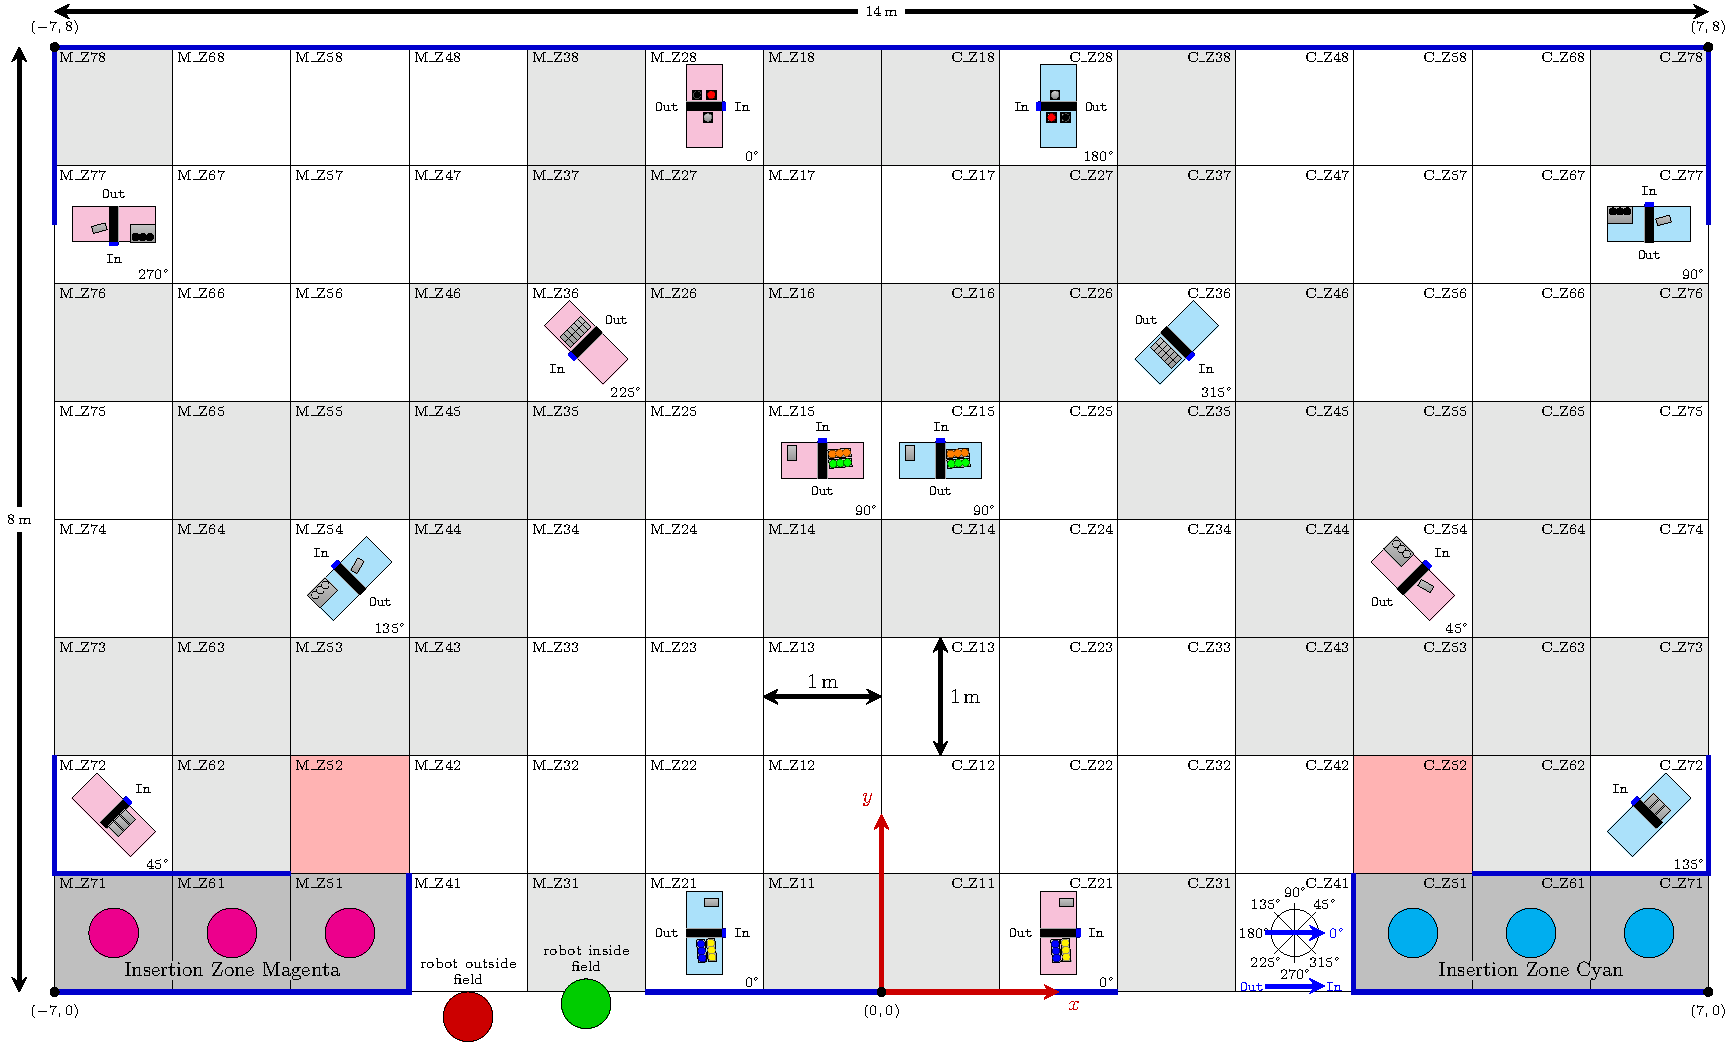
\includegraphics[width=\paperwidth, angle=-90, trim=0 0 0 0,]{field2022.pdf}
    \vspace{1ex}
    \caption{%
      Competition area for two teams: Squares indicate zones for possible
      machine placements, circles denote robots. Cyan and magenta are
      team assignment colors. Thick blue lines are wall elements.
      Dark gray areas are insertion areas where robots start. No machines may
      be placed in the vicinity of other machines (light gray areas) or at
      the insertion zone entrance (light red area).
    }
    \label{fig:competition-area}
\end{figure}
The competition area of the \ac{RCLL} has a rectangular shape. The field is
divided in square zones of \SI{1 x 1}{\metre}. %chktex 29
The zones of each field are named according to the following scheme:
A team prefix (``C-'' for cyan at the positive half of the X-axis, ``M-'' for
magenta at the negative half of the X-axs), ``Z'' to distinguish zone names,
and a grid coordinate form the name of a zone.
For example, The zone C-Z23 is a zone on the cyan primary half, which is
the second along the positive half of the X-axis and the third along the Y-axis.
Zones will not be physically represented or visible on the field.
They cannot be used for any other purpose than machine positioning.

The field is partially surrounded (at least 50\% but not more than 70\%)
by wall elements of at least \SI{0.5}{\metre} height.
Different machines are placed within the area, the constraints for
positioning them are given in \refsec{sec:machine-swapping}.
The \ac{RCLL} supports two kind of field layouts:
Firstly, a symmetrical one
with aspect ratio 1:2 intended for two teams to compete simultaneously
on the same area.
Secondly, a field with a squared layout that is intended for tasks,
where only one team is on the field at a time.
Fields also contain designated robot insertion areas, that are used as a
starting position for the robots when a game starts or a robot is inserted
into a running game. The usage of these areas is restricted to these purposes,
unless stated otherwise. The insertion area is also partially surrounded by
wall segments as shown in \reffig{fig:competition-area} and
\reffig{fig:competition-area-challenges}.
In the following, the different field layouts are presented.
The depicted field layouts are examples only, the actual
distribution and alignment of machines on the competition area will change
before the actual game starts and will be different for each game. Thus, teams
should focus on a generic approach for production, allowing for
dynamic adaptation of machine positions and alignments.

\subsection{Fields with Aspect Ratio 2 (Main Track Field)}
\label{sec:competition-area}
An example of a competition area for games on the main track is shown in
\reffig{fig:competition-area}, it
features a \SI{14 x 8}{\metre} large arena with 112 square zones %chktex 29
and with 14 randomly distributed machines (an identical set of 7 machines for
each team exclusively). % chktex 29

The distribution and alignment of all machines is axially symmetrical
on the y-axis. Thus, each team has similar conditions on both halves of
the competition field.
For details, see \refsec{sec:machine-swapping}.
The entire area is shared among both teams on the field and any robot may travel
anywhere at any time (while not obstructing for an extended period of
time or pushing other robots or machines).
However, there are primary sides (split along the y-axis) for each team where
a team's \textit{robot insertion area} is located.
We will refer to the side with positive coordinates on the x-axis as the
(primary) half of team cyan, and the side with negative coordinates on the
x-axis as the (primary) half of team magenta.

\subsection{Fields with Aspect Ratio 1 (Challenge Track Field)}
\label{sec:competition-area-aspect-ratio-1}
An example of a competition area with aspect ratio 1 is shown in
\reffig{fig:competition-area-challenges},
it spans a \SI{5 x 5}{\metre} large %chktex 29
arena with 25 square zones, where 3 machines are placed.

Only one team at a time competes on the area, the chosen team-color
does not matter. However, the field coordinates resemble the magenta halve
of the field, hence the coordinates on the x-axis of all zones are negative.
Teams can play as either cyan or magenta, as machine positions published by
the \ac{refbox} place the machines of both teams on the same location
(e.g., M-BS and C-BS are both placed at M-Z12 in the field of
\reffig{fig:competition-area-challenges}).

\begin{figure}[!ht]
    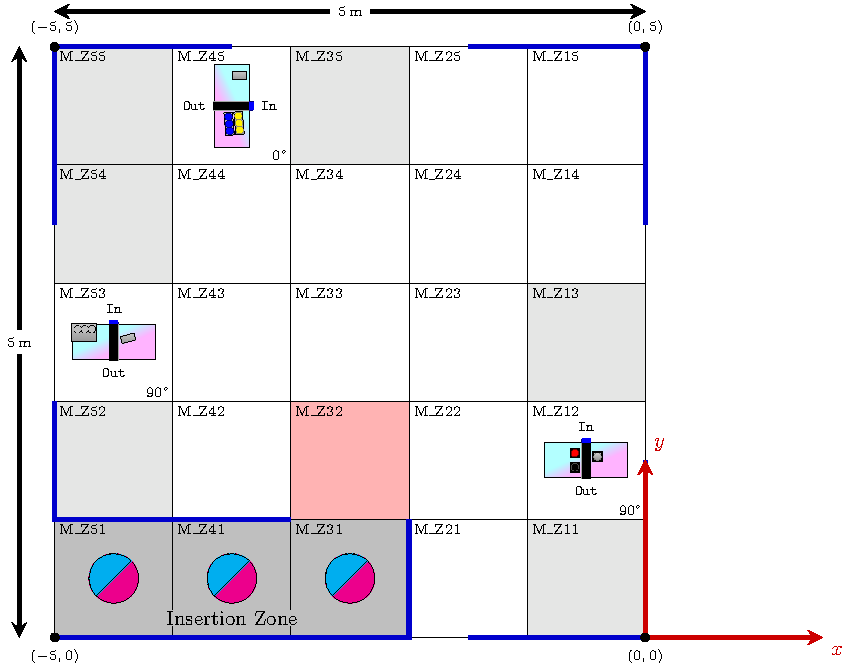
\includegraphics{challenge-field2021.pdf}
    \vspace{1ex}
    \caption{%
      Competition area for a field of the challenge track.
    }
    \label{fig:competition-area-challenges}
\end{figure}


\subsection{Moving on the Field}
\label{sec:field-movement}
The robots are free to move on the field. However, robots may not
leave the competition area (surrounded by the partial walls). That is, when
connecting all wall segments with the shortest possible edges, robots
may not move such that the base is fully outside this area. For
example, in \reffig{fig:competition-area}, the red robot is outside
the intended area and thus in an illegal position.

Robots that leave the competition area illegally are considered as
\emph{misbehaving robot} and punished accordingly
(cf.~\refsec{sec:misbehaving-robot}).

\section{Machines}
\label{sec:machines}
In the \ac{RCLL} 5 different types of production machines are
in use, each fulfilling a different role in the production process. Machines are
based on the \acf{MPS}\footnote{For
  more information see
  \url{http://www.robocup-logistics.org/links/festo-mps}.} by Festo
Didactic SE\@.
We use the terms \textit{MPS} and \textit{machine} interchangeably throughout
this rulebook.

Each \ac{MPS} shares the same basic layout as highlighted
in \reffig{fig:MPS-Layout}.
A movable rectangular trolley makes up the base of the machine.
A conveyer belt connecting the two short sides of
the machine is the main interaction point for robots.
Three colored signal lights are used to visually indicate the current state of
the machine.
Each machine type has additional individual application modules which provide
the different functionalities.


\begin{figure}[bh!]
  \centering
  \label{fig:MPS-Layout}
  \includegraphics[height=7cm]{MPS2015/MPS_Layout.jpg}
  \caption{General Machine Layout}
\end{figure}


Based on these shared properties, there are five kinds of machines:

\begin{description}
\item[\acf{BS}] acts as dispenser of base elements
  (\reffig{fig:BS}). The application modules are three magazines of
  base elements.
  %There is a single \ac{BS} per team.

\item[\acf{CS}] mounts a cap as the final step in production
  on an intermediate product (\reffig{fig:CS}). The application module
  is a vacuum pick \& place module. There is a slide to store at most
  one cap piece at a time. At the beginning this slide is empty and
  has to be filled in the following way.  A base element with a cap
  must be taken to the machine and is then unmounted and buffered in
  the slide. The cap is then mounted on the next intermediate product
  taken to the machine.
  %There are two \ac{CS} per team.

\item[\acf{RS}] mounts one colored ring out of two available
  colors on an intermediate product (\reffig{fig:RS}). Each \ac{RS} has two
  vacuum pick \& place units as application modules with separate
  unique colors which are determined new for each game. There is an
  additional pre-fill slide which is used for some colors (specified
  anew for each game) to add base elements.
  %There are two \ac{RS} per team.

\item[\acf{SS}] provides 48 slots of storage divided into
  6 layers (\reffig{fig:SS_portrait}).
  The Storage Station initially provides one pre-stored sample of each possible
  $C_0$ configuration (one per layer).

\item[\acf{DS}] Accepts completed products. The stations contains
  three slides (\reffig{fig:DS}). The delivered products are verified by either
  the referees or an automated external vision system.
  %There is one \ac{DS} per team.
\end{description}

\noindent
Machines of type \ac{CS} and \ac{RS} are called production machines as they
perform refinement steps on a workpiece during the production
phase. Processing times are outlined in \reftab{tab:processing-times}.

\begin{figure}[bh!]
\centering
% \subfigure[General Machine Layout]{%
%     \label{fig:MPS-Layout}
%     \begin{minipage}[b]{1\linewidth}
%         \centering
%         \includegraphics[height=7cm]{MPS2015/MPS_Layout.jpg}
%     \end{minipage}
% }
\quad
\subfigure[Base Station]{%
  \label{fig:BS_portrait}%
  \label{fig:BS}
  \begin{minipage}[b]{0.3\linewidth}
    \centering
    \includegraphics[height=6cm]{MPS2015/BS_portrait.png}
  \end{minipage}
}
\quad
\subfigure[Cap Station]{%
    \label{fig:CS_portrait}
    \label{fig:CS}
    \begin{minipage}[b]{0.3\linewidth}
        \centering
        \includegraphics[height=6cm]{MPS2015/CS_portrait.png}
    \end{minipage}
}
\quad
\subfigure[Ring Station]{%
    \label{fig:RS_portrait}
    \label{fig:RS}
    \begin{minipage}[b]{0.3\linewidth}
        \centering
        \includegraphics[height=6cm]{MPS2015/RS_portrait.png}
    \end{minipage}
}
\quad
\subfigure[Storage Station]{%
    \label{fig:SS}
    \label{fig:SS_portrait}
    \begin{minipage}[b]{0.3\linewidth}
        \centering
        \includegraphics[height=6cm]{MPS2015/SS_portrait.jpg}
    \end{minipage}
}
\quad
\subfigure[Delivery Station]{%
    \label{fig:DS}
    \begin{minipage}[b]{0.3\linewidth}
        \centering
        \includegraphics[height=6cm]{MPS2015/DS_Input.png}
    \end{minipage}
}
\vspace{-1ex}
\caption{The different \ac{MPS} stations}
\end{figure}

\begin{table}[!tb]
    \centering
    \mytable{
        \begin{tabularx}{\linewidth}{l|l|X}
            Type & Distribution & (Final) processing time[s]\\\hline
            \acf{BS} & 1 per team & minimum physical time\\
            \acf{CS} & 2 per team & $t_2 = \SItextrange{15:25}{\sec}$\\
            \acf{RS} & 2 per team &$t_3 = \SItextrange{40:60}{\sec}$\\
            \acf{SS} & 1 per team & minimum physical time\\
            \acf{DS} & 1 per team &$t_5 =\SItextrange{20:40}{\sec}$
        \end{tabularx}
    }
    \caption{\ac{MPS} type, distribution and processing times}
    \label{tab:processing-times}
\end{table}

\subsubsection{Physical Description of Machines}

The stations have a rectangular base shape of \SI{0,35 x 0,7}{\metre}% chktex 29
with a height of about \SI{1}{\metre} depending on machine type.
A machine is movable by four wheels with \SI{0.1}{\metre} clearance.
Both narrow sides of the trolley are closed by plexiglas and have a handle.
All physical interfaces like conveyor belt inputs and outputs, shelves, and
slides for additional bases on ring stations are accessible at
\SI{89.8}{\centi\metre} height\footnote{Note however, that due to small
  variances and unevenness in the floor there may likewise be small variances
  in the working height of some or all parts of a station.}.
Working space between guiding lanes is \SI{4.5}{\centi\metre}. Setup lanes and
shelves feature approximately the same space for handling and
adjusting. All diffuse sensors (input side) have been removed to allow
for infrared-emitting cameras.  To simplify the delivery on the belt,
each machine will be equipped with a narrowing cone on its input side
(\reffig{fig:narrow-cone}).  You can order them from Festo Didactic SE
(C. Deppe) or download the STL model file from the \ac{RCLL} site.
\begin{figure}
    \includegraphics[height=8cm]{narrowConeSketch.jpg}
\caption{Narrowing cone}
\label{fig:narrow-cone}
\end{figure}
% Still unclear, thus commenting out.
% If observed from the output side of machines (where the signal unit
% is placed) the conveyor space opens up at half of the aluminum
% profile thus starting at \SI{0,35}{\metre}.
%\begin{figure}[b!]
%    \centering
%    \includegraphics[height=7cm]{MPS2015/MPS_Layout.jpg}
%
%    \caption{General Machine Layout}
%    \label{fig:MPS-Layout}
%\end{figure}

\subsubsection{Machine Positioning}
\label{sec:machine-swapping}
The zones and rotations for the \ac{MPS} will be randomly chosen by the
\ac{refbox}\footnote{It is also possible to store and retrieve field layouts
  with the \ac{refbox}, which is useful for testing purposes or if a game needs
  to be restarted. See the \ac{refbox} configuration options in the wiki
for details.}.
Each game will have a new randomly generated field layout, the referees will
place the \ac{MPS} in the middle of the zone with given rotation at there
best effort but errors of the positioning should be expected.

A \ac{MPS} can generally  be placed in any zones except those at the
entrance of the insertion area (the light red areas in
\reffig{fig:competition-area} and \reffig{fig:competition-area-challenges}).
These zones are needed to enter the field. Each \ac{MPS} has one out of 8
possible orientations, starting at \ang{0} with steps of \ang{45}
Intuitively, the different orientations are shown in the pictogram in
zone C\_Z41 of \reffig{fig:competition-area}, where
the tip of the blue arrow represents the input side of a machine and points
towards the respective rotation (\ang{0} in that figure).
Formally, to denote
the orientation  we assign a local right-handed coordinate system to
each \ac{MPS} station. The x-axis is given by the conveyor pointing from
the output to the input. The origin is the center point of the
conveyor. The orientation is then the relative rotation of the local
\ac{MPS} system compared to the fixed field coordinate system. For example,
at an \ac{MPS} orientation of \ang{0}, its local coordinate system is
aligned with the field (in terms of orientation). Furthermore, an \ac{MPS}
at an orientation of \ang{90} will be rotated counter-clockwise a
quarter turn compared to the field system.

To ensure fairness, positions and orientations of the machines are mirrored
along the field's y-axis. There are two cases that need to be handled
separately. First, machines in a cell not adjacent to the wall, and machines of
types \ac{BS}, \ac{DS}, and \ac{SS} (even when adjacent to the wall) are
mirrored according to \reftab{tab:mirror-a}. Second, \ac{CS} and \ac{RS}
stations must be handled slightly different,
if oriented next to a wall or field border
(e.g., zones C-Z*1, C-Z*8, C-Z7*, M-Z*1, M-Z*8 and M-Z7* in
\reffig{fig:competition-area}).
The reason being, that the shelf and slide of these stations are
offset sideways at the input side. This might lead to the situation that for one
team the shelf is close to the wall, and for the other it is not. To remedy this
problem, the \ac{RS} and \ac{CS} machines adjacent to a wall will always
be placed such that the shelf or slide is on the farther end with respect
to the wall.
For example, in \reffig{fig:competition-area}, the magenta \ac{CS}
in M-Z77 with a rotation of \ang{270}. Were this setup mirrored, the shelf
on the cyan \ac{CS} in C-Z77 would be close to the wall.
Instead, it has a different orientation violating the y-symmetry
but allowing for easier access to the shelf.

\begin{wrapfigure}[10]{R}{0.2\linewidth}
  \centering
  \vspace{-2.1ex}
  \mytable{
    \begin{tabularx}{\linewidth}{
      >{\raggedleft\arraybackslash}X|>{\raggedleft\arraybackslash}X
    }
      Cyan & Magenta \\ \hline
      \ang{0}&\ang{180}\\
      \ang{45}&\ang{135}\\
      \ang{90}&\ang{90}\\
      \ang{135}&\ang{45}\\
      \ang{180}&\ang{0}\\
      \ang{225}&\ang{315}\\
      \ang{270}&\ang{270}\\
      \ang{315}&\ang{225}\\
	\end{tabularx}}%
  \makeatletter%
  \def\@captype{table}%
  \makeatother%
  \caption{\ac{MPS} orientation mapping during mirroring}
  \label{tab:mirror-a}
\end{wrapfigure}

\begin{figure}[tb]
    \centering
    \subfigure[
      For rotations with \ang{0}, \ang{90}, \ang{180} or \ang{270}.
      \ac{BS}, \ac{CS}, \ac{RS}, and \ac{SS} block the zones close to the
      input as well as the output. \ac{DS} blocks the zones close to the input.
    ]{
        \label{fig:zone-mps-rotation-straight}%
        \centering
        \includegraphics[width=\textwidth]{bZones1.pdf}
    }
    \quad
    \subfigure[
      For rotations with  \ang{45}, \ang{135}, \ang{225} and \ang{315}.
      \ac{BS}, \ac{CS}, \ac{RS}, and \ac{SS} block the zones close to the
      input as well as the output. \ac{DS} blocks the zones close to the input.
    ]{
        \label{fig:zone-mps-rotation-odd}
        \centering
        \includegraphics[width=\textwidth]{bZones2.pdf}
    }
    \caption{
      Blocked zones regarding the \ac{MPS} rotation (red zones must not
      be used as position for other machines and must be located inside
      the competition area).
    }
    \label{fig:zone-mps-blocked}
\end{figure}
For placing of machines, the \ac{refbox} will take care of the
necessary constraints to ensure that all in- and output sides, shelves
and slides are reachable. That
is, a path to each blocked zone (see \reffig{fig:zone-mps-blocked}) must exist
from any unoccupied or blocked zone of the field. If a machine is rotated with
\ang{0}, \ang{90}, \ang{180} or \ang{270} the zones in front the input and
output side are blocked as well (\reffig{fig:zone-mps-rotation-straight}).  For
machines with rotations \ang{45}, \ang{135}, \ang{225} and \ang{315} three zones
in front of each input and output side are blocked
(\reffig{fig:zone-mps-rotation-odd}). No \ac{MPS} nor blocked zones for
another \ac{MPS} may be placed in a blocked zone.
All blocked zones of any \ac{MPS} must be located
within the competition area. Furthermore, only two machines will ever be placed
next to each other, a third machine will only be placed with at least one empty
zone in-between.


\subsubsection{Markers}
\label{sec:markers}
\begin{table}[b!]
  \centering
  \begin{tabular}{|l|c|c|c|c|l|}
    \hline
    && \multicolumn{2}{c|}{Input}
    & \multicolumn{2}{c|}{Output}
    \\
    \hline
    &Machine & ID & Tag & ID & Tag
    \\
    \hline
    &&&&&\\[-2ex]
    \multirow{7}{*}{\rotatebox{90}{\bfseries Cyan\hspace{3.75cm}}}
    & \ac{CS} 1 & 102
           & \parbox[c]{1.2cm}{
               
\includegraphics[width=1.2cm]{markers/figure_102}}
           & 101
           & \parbox[c]{1.2cm}{
               
\includegraphics[width=1.2cm]{markers/figure_101}}
    \\[2.5ex]
    & \ac{CS} 2 & 104
           & \parbox[c]{1.2cm}{
               
\includegraphics[width=1.2cm]{markers/figure_104}}
           & 103
           & \parbox[c]{1.2cm}{
               
\includegraphics[width=1.2cm]{markers/figure_103}}
    \\[2.5ex]
    & \ac{RS} 1 & 112
           & \parbox[c]{1.2cm}{
               
\includegraphics[width=1.2cm]{markers/figure_112}}
           & 111
           & \parbox[c]{1.2cm}{
               
\includegraphics[width=1.2cm]{markers/figure_111}}
    \\[2.5ex]
    & \ac{RS} 2 & 114
           & \parbox[c]{1.2cm}{
               
\includegraphics[width=1.2cm]{markers/figure_114}}
           & 113
           & \parbox[c]{1.2cm}{
               
\includegraphics[width=1.2cm]{markers/figure_113}}
    \\[2.5ex]
    & \ac{BS} & 122
         & \parbox[c]{1.2cm}{
             
\includegraphics[width=1.2cm]{markers/figure_122}}
         & 121
         & \parbox[c]{1.2cm}{
             
\includegraphics[width=1.2cm]{markers/figure_121}}
    \\[2.5ex]
    & \ac{DS} & 132
         & \parbox[c]{1.2cm}{
             
\includegraphics[width=1.2cm]{markers/figure_132}}
         & 131
         & \parbox[c]{1.2cm}{
             
\includegraphics[width=1.2cm]{markers/figure_131}}
    \\[2.5ex]
    & \ac{SS} & 142
         & \parbox[c]{1.2cm}{
             
\includegraphics[width=1.2cm]{markers/figure_142}}
         & 141
         & \parbox[c]{1.2cm}{
             
\includegraphics[width=1.2cm]{markers/figure_141}}
    \\[2.5ex]
    \hline
  \end{tabular}
  \hfill
  \begin{tabular}{|l|c|c|c|c|c|}
    \hline
    && \multicolumn{2}{c|}{Input} & \multicolumn{2}{c|}{Output}\\\hline
    &Machine & ID & Tag & ID & Tag\\\hline
    &&&&&\\[-2ex]
    \multirow{7}{*}{\rotatebox{90}{\bfseries Magenta\hspace{3.75cm}}}
    & \ac{CS} 1 & 202
           & \parbox[c]{1.2cm}{
               
\includegraphics[width=1.2cm]{markers/figure_202}}
           & 201
           & \parbox[c]{1.2cm}{
               
\includegraphics[width=1.2cm]{markers/figure_201}}
    \\[2.5ex]
    & \ac{CS} 2 & 204
           & \parbox[c]{1.2cm}{
               
\includegraphics[width=1.2cm]{markers/figure_204}}
           & 203
           & \parbox[c]{1.2cm}{
               
\includegraphics[width=1.2cm]{markers/figure_203}}
    \\[2.5ex]
    & \ac{RS} 1 & 212
           & \parbox[c]{1.2cm}{
               
\includegraphics[width=1.2cm]{markers/figure_212}}
           & 211
           & \parbox[c]{1.2cm}{
               
\includegraphics[width=1.2cm]{markers/figure_211}}
    \\[2.5ex]
    & \ac{RS} 2 & 214
           & \parbox[c]{1.2cm}{
               
\includegraphics[width=1.2cm]{markers/figure_214}}
           & 213
           & \parbox[c]{1.2cm}{
               
\includegraphics[width=1.2cm]{markers/figure_213}}
    \\[2.5ex]
    & \ac{BS} & 222
         & \parbox[c]{1.2cm}{
             
\includegraphics[width=1.2cm]{markers/figure_222}}
         & 221
         & \parbox[c]{1.2cm}{
             
\includegraphics[width=1.2cm]{markers/figure_221}}
    \\[2.5ex]
    & \ac{DS} & 232
         & \parbox[c]{1.2cm}{
             
\includegraphics[width=1.2cm]{markers/figure_232}}
         & 231
         & \parbox[c]{1.2cm}{
             
\includegraphics[width=1.2cm]{markers/figure_231}}
    \\[2.5ex]
    & \ac{SS} & 242
         & \parbox[c]{1.2cm}{
             
\includegraphics[width=1.2cm]{markers/figure_242}}
         & 241
         & \parbox[c]{1.2cm}{
             
\includegraphics[width=1.2cm]{markers/figure_241}}
    \\[2.5ex]
    \hline
  \end{tabular}
  \vfill
  \vspace{0.5cm}
  \begin{tabular}{|c|c|c|}
    \hline
    Machine & ID & Tag \\\hline
    &&\\[-2ex]
     \ac{UMPS} & 301
           & \parbox[c]{1.2cm}{
               
\includegraphics[width=1.2cm]{markers/figure_301}}
    \\[2.5ex]
    \hline

  \end{tabular}
  \caption{Machine tags are ARUCO tags (from the original ARUCO dictionary,
  $5\times 5$ bits, 1024 markers) with the given IDs.}
  \label{tab:markers}
\end{table}
Each machine can be equipped with two \emph{markers} based on ARUCO AR tags,
one placed on the input, another one on the output side.
Teams can choose whether uniquely identifying markers should be added to their
machines or not.
In the main track of the \ac{RCLL}, where two teams compete on the same playing
field, \acl{UMPS} markers may be used for machines of a team that
does not require markers, if the opposing team relies o the presence of markers.

Markers will be
horizontally centered below the conveyor belt. The vertical distance
between the tag's upper edge and the conveyor belt will be about
\SI{35}{\centi\metre}. The markers will be mounted at the same
position on all machines in a best effort fashion, but teams should expect
slight deviations to their exact position.
The markers are available for printing on the rulebook github\footnote{
  \url{https://github.com/robocup-logistics/rcll-rulebook/tree/master/markers/numbered_markers.pdf} % chktex ignore-long-line
}.

\subsection{Mockup Machines}
\label{sec:mockup-machines}
In case no real \ac{MPS} stations are available, replications
(so called \emph{mockup machines}) may be used, that do not need to
physically perform the respective production steps. Instead, that work may
be carried out by a human supervisor (see \refsec{sec:during-match}).
The minimum requirements for a mockup machine are specified in the following.

Mockup machines are required to have the same box-like base shape as specified
in the \ac{RCLL} rulebook.
Additionally, the following parts need to be mounted:
\begin{itemize}
	\item a model of the conveyor belt
	\item a shelf on the front right side of the box on stations replicating a
		CS
	\item either a shelf, a slide or a conveyor belt on the front right side
of the box, such that it is accessible from the front on stations replicating a
		\ac{RS}
\end{itemize}
Models for a conveyor belt, shelf and slides can be found in the
\ac{RCLL} rulebook repository\footnote{\url{https://github.com/robocup-logistics/rcll-rulebook/tree/master/mock_up_models}}. % chktex ignore-long-line

The building materials for the models must be opaque, but may have any color.

\section{Game Play}
At the beginning of each match, the \ac{refbox} must be configured according to
the game mode specification.
To guide the match, the \ac{refbox} utilizes different phases,
which are outlined in the following sections. Within the different game modes in
the \ac{RCLL} (see \refsec{sec:tournament-main} and
\refsec{sec:tournament-challenges}), different phases might be utilized.
Regardless of the game mode, all matches will
start at the exact time scheduled by the Organizing Committee in the setup phase
(cf.~\refsec{sec:setup-phase}).


\subsection{Setup Phase}
\label{sec:setup-phase}
Once the \ac{refbox} is initialized, it switches to the setup phase.
All robots which are to
participate in the game need to be in the insertion area during the setup phase
(not in the game area where the machines are located).
During the setup phase, the \ac{refbox} announces the layout of the competition
area, including the ring colors assigned to the ring stations to the referees.
Machine positions are not communicated to the robots yet.
The competing team(s) may use the setup phase to start up their  %chktex 36
robots and to fill their machines (see \refsec{sec:machine-refill}).
Once the setup phase ends, no more interference (physically or remotely) with
the robot is allowed. The robot(s) must react to the \ac{refbox} %chktex 36
game state messages and start the game play autonomously.
The \ac{refbox} will automatically end the setup phase after 5 minutes.
Production phase follows.

\subsection{Production Phase}
\label{sec:production-phase}
During the production phase machines can be used to assemble products
according to dynamically arriving orders.
The \ac{refbox} publishes information regarding products and machines.
This includes configured colors at the ring stations and their
prices.
Depending on the played format, machine zones and orientations may be announced
as well.
A minimum of zero points will be accounted for the production phase.

\subsubsection{Exploration Period}
\label{sec:exploration-period}

The \ac{refbox} is tasked with distributing machine information
(including position) during the game to the robots of each team.
Depending on the game mode, complexity might be increased by using an
\textit{exploration period} at the beginning of the production phase.
During this period, the positions of the machines won't be announced and the
robots of both teams can roam the environment and report their (and only their)
machines to the \ac{refbox}.
Correctly reported machines will be rewarded with points and can
be used for production. Machines can be identified through two different ways:
either by relying on the provided unique tags, or by using visual object
classification methods.
Teams are free to choose which method they will use, but the
decision needs to be announced to the judges before the machine setup begins.
Depending on the team's choice, the machines of a team will either be equipped
with unique tags (should the tag based approach be chosen) or \ac{UMPS} tags.
Points will be awarded for correct discoveries regardless of the chosen
difficulty.
The scoring is shown in \reftab{tab:scoring}.

Moving or processing workpieces at an \ac{MPS} is explicitely
allowed during the exploration period.
As soon es the necessary machines have been
correctly identified and reported to the \ac{refbox},
production of announced orders or machine preparation can immediately begin.

Reports are issued to the refbox using a \emph{MachineReport message}.
For each machine, identified by its name, both its zone and its orientation
(in degrees) can be explored.
Both properties can be submitted at the same time in one message or be split up
into multiple messages.
The refbox accepts only the first submitted value for each property.
For a detailed description of the message please refer to the \ac{refbox}
wiki\footnote{\url{https://github.com/robocup-logistics/rcll-refbox/wiki/Communication-Protocol}}. % chktex ignore-long-line

The exploration period ends automatically after the time span has passed.
Its end is marked by the distribution of machine position information from the
\ac{refbox} to the robots.

\subsubsection{Workpieces}
\label{sec:workpieces}
Workpieces denote raw materials that need to be refined through production
steps.
They consist of the following elements:
\begin{description}
\item[Base] The base is the lowermost element of each workpiece.
  Bases are dispensed by the \acf{BS} and bases with mounted
  caps are available on the \acf{CS}. Bases are available in
  the colors red, black, silver, and transparent. Transparent bases
  are to be used and only used on \ac{CS} shelves
  (cf.~\refsec{sec:production-machines-production}), they cannot be
  used as a workpiece for production. They may, however, be used to
  provide additional bases required by an \ac{RS}, stored on a team's \ac{CS}
  shelf, or recycled at the \ac{DS}.
\item[Ring] Rings are mounted in intermediate production steps at the \acf{RS}.
\item[Cap] Caps are the topmost element of each workpiece. They are
  obtained by taking pre-assembled base-cap combinations available on
  the shelf to the \acf{CS}. Caps can be black or gray.
\end{description}

\begin{figure}[ht]
  \centering
  \subfigure[Workpiece base elements and caps.]{
    \label{fig:workpieces-base-elements}%
    \centering
    \includegraphics[height=5cm]{figures/workpieces}
  }
  \quad
  %
  \subfigure[Renderings of intermediate rings (rings are colored in
  competition).]{
    \label{fig:workpieces-rings}%
    \centering
    \hspace{6mm}
    \includegraphics[height=3cm]{figures/rings}
    \hspace{6mm}
  }
  \quad
  \subfigure[Prototype base barcode]{\label{fig:barcode}%
%TODO: WTF is this figure, the rings are white....
    \includegraphics[height=3cm]{figures/barcode-base}
  }
  \caption{Workpiece elements and product example.}
  \label{fig:workpieces}
\end{figure}

\paragraph{Barcodes.}
All bases are labeled with a horizontally encircling, white glossy tag
covering about 50 percent of the bases height (from the center)
containing a white reference area as well as an identifying
barcode. Each base is equipped with a unique ID\@. \reffig{fig:barcode}
shows a prototype of a barcode labeled workpiece.

The barcodes can be scanned at each station via attached barcode scanners and
communicated to the \ac{refbox}.
The \ac{refbox} can use this information to track assembly
processes, i.e., to determine the state of a workpiece.
However, this feature is only available, if the scanners are attached
to the machines, which may not be the case as this system is still under
evaluation.

\subsubsection{Production, Color Complexities, and Additional Bases}
\label{sec:production-complexities}
The product portfolio comprises many different variants and is
categorized by the four available \emph{product complexity} levels
shown in \reffig{fig:production-complexities}. The lowest complexity
$C_0$ consists of just a base and a cap and requires to load the \ac{CS}
with the proper cap color and then processing a properly colored base
at that machine. The highest complexity $C_3$ requires a base with
three mounted rings and a cap. For a product, the colors of base,
rings, and cap as well as the order of the rings are of importance.

Depending on the ring color, the robot may need to deliver one or more
\emph{additional bases} to a \ac{RS} first in order to enable it to mount
the ring. We therefore distinguish \emph{color complexities} as $CC_0$, $CC_1$,
and $CC_2$ depending on whether zero, one, or two additional bases are
required for a color.

Each order will consist of the product variant to
produce, the amount thereof, and a delivery time slot. An order
therefore specifies a production chain to be accomplished for
fulfillment. \reffig{fig:production-chains} shows some example
production chains of the four different complexities
(cf.~\reffig{fig:production-complexities}).

Products retrieved from the Storage Station may be used only for
$C_0$ orders with a requested quantity equal to or greater than two.
An order can be \emph{competitive} or \emph{non-competitive}. For a competitive
order, the team that delivers it first will get extra points
(cf.~\refsec{sec:production-scoring}).
For a non-competitive order, each team scores independently of the other team.

\begin{figure}
  \ffigbox{%
    \centering

    \hfill
    \subfigure[$C_0$]{\label{fig:prod-compl-0}%
      
\includegraphics{products/c0_black_gray}
    }
    \hfill
    \subfigure[$C_1$]{\label{fig:prod-compl-1}%
      
\includegraphics{products/c1_red_blue_black}
    }
    \hfill
    \subfigure[$C_2$]{\label{fig:prod-compl-2}%
      
\includegraphics{products/c2_silver_blue_green_black}
    }
    \hfill
    \subfigure[$C_3$]{\label{fig:prod-compl-3}%
      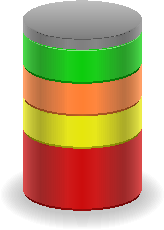
\includegraphics{products/c3_red_yellow_orange_green_gray}
    }
    \hfill\,

}{%
  \caption{Products are composed of a base element and a cap with
    zero, one, two, or three intermediate rings representing the
    product complexity. The complexity level is stated as the number of
    required intermediate rings. The base element colors are red,
    black, and silver, the ring colors are blue, green, yellow, and
    orange, and the cap colors are either gray or black.}
  \label{fig:production-complexities}
}
\vspace{-1mm}
\end{figure}

\begin{figure}[p]
    \centering
    \subfigure[Production of complexity $C_0$ received from a \ac{SS}.]{
      \label{fig:prod-chain-C0-SS}%
      \begin{minipage}{1.0\linewidth}
        \centering
        \includegraphics[scale=0.8,page=5]{production-examples}
      \end{minipage}
    }
    \subfigure[Production of complexity $C_0$ as shown in
    \reffig{fig:prod-compl-0}.
    A cup must be buffered at the
    \ac{CS} (red path) before a cap can be mounted on the product (green path).
    The remaining cap-less carrier is not needed for the product.
    ]{
      \label{fig:prod-chain-C0}%
      \begin{minipage}{1.0\linewidth}
        \centering
        \includegraphics[scale=0.8,page=1]{production-examples}
      \end{minipage}
    }
    \subfigure[Production of complexity $C_1$ according to
    \reffig{fig:prod-compl-1}.]{\label{fig:prod-chain-C1}%
      \begin{minipage}{1.0\linewidth}
        \centering
        \includegraphics[scale=0.8,page=2]{production-examples}
      \end{minipage}
    }
    \subfigure[Complexity $C_2$ (cf. \reffig{fig:prod-compl-2}).
    The second ring requires an additional base (of any color) for the
    green ring.
    The cap-less carrier is used as payment in this example.
    ]{\label{fig:prod-chain-C2}%
      \begin{minipage}{1.0\linewidth}
        \centering
        \includegraphics[scale=0.8,page=3]{production-examples}
      \end{minipage}
    }

    \subfigure[Production of the highest complexity $C_3$ according to
    \reffig{fig:prod-compl-3}.
    Note that two additional bases (of any color) are required to pay for
    the green ring and another one is needed for for the orange ring.
    A cap-less carrier (red arrow), a capcarrier (blue arrow) and a fresh base
    from the \ac{BS} (brown arrow) are used in this example to fulfill the
    payments.
    ]{\label{fig:prod-chain-C3}%
      \begin{minipage}{1.0\linewidth}
        \centering
        \includegraphics[scale=0.8,page=4]{production-examples}
      \end{minipage}
    }
  \caption{Production Chains of four example products
    (cf. \reffig{fig:production-complexities}). Green arrows show the product
    path from start to delivery, red arrows show the path of a capcarrier that
    is used to buffer the \ac{CS}.
    \emph{Note that this is a particular
      example. The actual production chains and requirements for
      additional BEs are determined randomly by the \ac{refbox} for
      each game and steps such paying BEs can be accomplished in different
      ways.}}
  \label{fig:production-chains}
\end{figure}

\subsubsection{MPS --- During Production Phase}
\label{sec:production-machines-production}
In the production phase a production machine performs refinement steps on
a product such as mounting an additional ring or a cap. Machines
operate in a transaction style. That is, before using a machine it
must be prepared for a specific mode. Then the input products can be fed
into the machine and the refinement step commences. Eventually, after
the production period is completed, the resulting product is delivered
on the output lane.

A light signal mounted near the output lane
(cf. \refsec{sec:machines}) indicates the state of the machine.
The light signals are summarized in
\reftab{tab:machine-lights}.

In the production phase, machines must be prepared to be used by instructing
the refbox. This applies to all machine types.
If a product from the input is required for the processing step
(\ac{DS}, \ac{CS}, \ac{RS} and a storage operation at the \ac{SS}),
then the conveyor belt is started
after receiving a prepare message. If no workpiece reaches the
machine operating point (indicated through the middle belt sensor)
within \SI{45}{\second}, the machine goes to a temporary out-of-order
state (cf.~\refsec{sec:broken-machine}).
The \ac{BS} and the retrieval operation at the \ac{SS} cause
the requested workpiece to be dispensed upon receiving a prepare message.
After performing an operation at the \ac{BS}, \ac{CS}, \ac{RS} or the \ac{SS}
(in case of a retrieval) the conveyor belt is started.
If no workpiece reaches the destination
point (indicated through the output belt sensor, or in case of the \ac{BS}
either the input or output belt sensor) within \SI{90}{\second},
the machine goes in a temporary out-of-order state
(cf.~\refsec{sec:broken-machine}).
The workpiece may remain on the machine for an arbitrary time after the
operation is completed.

The following describes the communication and reactions of the
machines during the production phase. For the actual messages we refer
to the \ac{refbox} documentation (see \refsec{sec:task}).

\smallskip

\noindent\textbf{\acl{BS}}
The \ac{BS} prepare message denotes the color of the base element that should
be dispensed. After receiving the message, the \ac{refbox} will instruct
the \ac{MPS} to immediately provide a base of the desired color.

\noindent\textbf{\acl{RS}}
The \ac{RS} prepare message must state which of the two colors to prepare and
retrieve. Each \ac{RS} is responsible for two specific colors. Some colors
require loading the \ac{RS} with additional bases
(cf.~\refsec{sec:production-complexities}). If the desired color requires
additional bases, the machine expects to receive them first.
Once the required number of
additional bases has been received, the intermediate product can be
fed into the machine. It receives a ring of the desired color and
moves the processed product to the output.

\noindent\textbf{\acl{CS}}
The \ac{CS} prepare message initiates either the retrieval or the mounting of
a cap. For retrieving a prepared base (with a cap mounted on top) from
the machine's shelf must be fed into the machine. All base elements
prepared on the shelf are specially colored workpieces (clear). The
machine will take the cap off the base and buffer it on the slide,
releasing the decapped base to the output side. This base can only be
used for providing an additional base to an \ac{RS} (see below), reuse by
placing it back on the shelf, or discarding it at the \ac{DS}.  For
mounting a cap, a workpiece (without cap) must be provided onto which
the cap is mounted.

\noindent\textbf{\acl{DS}}
The \ac{DS} prepare message denotes the order ID of the product
that is delivered.
The \ac{DS} will consume any workpiece provided,
but points can only be scored if the \ac{DS} has been properly prepared.

\noindent\textbf{\acl{SS}}
The \ac{SS} prepare message denotes the storage place (shelf and slot number)
and the type of the operation that should be performed.
The \ac{SS} consists of six shelves with eight slots each. \reffig{fig:ss-shelf}
depicts how positions are mapped to their respective shelf and slot numbers
$(x,y),x\in[0,5],y\in[0,7]$.
Accessing a slot $(x,y), y\in\{1,3,5,7\}$ in the back of a shelf while slot
$(x,y-1)$ is occupied causes the \ac{SS} to relocate the product at $(x,y-1)$
to a randomly chosen accessible position before processing the instruction.
If all other free positions are located in the back and
are also blocked by products stored in front of them, then one of those free
positions $(x^\prime,y^\prime)$ is chosen and
$(x^\prime,y^\prime-1)$ is relocated to $(x^\prime,y^\prime)$, before
relocating $(x,y-1)$ to $(x^\prime,y^\prime)$.
Descriptions can be added to the prepare messages when storing workpieces.
These descriptions are attached to the position of the workpiece and updated
automatically when relocating operations happen.
Each team receives the storage status for their respective \ac{SS}
periodically, including the corresponding descriptions at each position.
Positions and configurations of pre-stored products are also announced through
storage status messages.
Note the costs for using the \ac{SS} outlined in
\refsec{sec:production-scoring}.


\begin{figure}[ht]
  \centering
    \includegraphics{figures/storage-shelf.pdf}
    \caption{The bottom-most \ac{SS} shelf. Position $(x,y)$ consists of
      shelf number $x$ and slot number $y$.
    Shelves are numbered in ascending order from bottom to top.}
    \label{fig:ss-shelf}
\end{figure}

\medskip
The preparation and use of a machine follows a transaction style. Once the
machine has been prepared, the full cycle can be completed (committed).
There may be only one transaction running at a time. If a
second preparation is performed the machine will
be temporarily broken, which causes it to recover to a determined state.
An \ac{MPS} may be reset by a team at any time by a dedicated msg.
This causes the \ac{MPS} to go into the broken state as well.

\begin{table}
  \begin{tabular}{c|c|c||l}
    \hline
    \multicolumn{3}{c||}{\bf{Light Signals}} &
    \multicolumn{1}{c}{\bf{Description}} \\\cline{1-3}
    RED & YELLOW    & GREEN & \\\hline
    ON    &       &       & Machine is DOWN, temporarily unavailable \\
          & ON    &       & Report received, not processed yet \\
          &       & ON    & Machine is IDLE and usable  \\
          &       & BLINK & Machine is PREPARED  \\
          & BLINK &       & Zone reported correctly \\
    ON    & ON    &       & Zone reported wrongly \\
          & ON    & ON    & Machine is processing \\
    ON    & BLINK &       & Rotation reported wrongly \\
          & ON    & BLINK & Machine is READY-AT-OUTPUT \\
    BLINK & BLINK &       & Machine was wrongly instructed, it is currently
    BROKEN \\
          & BLINK & BLINK & Machine is WAIT-IDLE, soon to be IDLE again \\
  \end{tabular}
  \caption{Light codes for each machine status during the production phase.}
  \label{tab:machine-lights}
\end{table}

\subsubsection{Broken Machine Downtime}
\label{sec:broken-machine}
If a machine is improperly instructed or used, or a reset message has
been sent, the machine will go into a failure state. The machine cannot be
used for 30 seconds and until repaired.
That is, if damage was
inflicted on the machine or the referee needs longer to repair the
machine the game continues and the machine will be offline for a
longer time. Any production that was running will be aborted and any
product which was being processed is no longer available and will be
removed by the referee. Any additional bases or caps buffered at the machine
will be void and the points gained removed. For storage stations, no
slot is refilled, the load status remains exactly as before the broken
state. The downtime is indicated by a flashing red light.


\subsubsection{Scheduled Machine Downtime}
\label{sec:out-of-order}
Depending on the game format, the \ac{refbox} may take down \ac{RS} and \ac{CS}
machines at random. If two teams play at the same time, then the same machines
for both teams are affected in the same time window.
The machines affected will remain out of order for 30 to 60
seconds. Every machine can only be forced out of order once per
match. If a machine turns offline during processing of a product it will
afterwards resume the process (extending the overall processing time
by the duration of the time spent offline). The downtime is indicated by a
steady red light.
Base elements fed into the machine while out-of-order are
accepted when the machine gets back online, with the same constraints
mentioned in \refsec{sec:production-machines-production}.



\subsection{Task Fulfillment and Scoring}
\label{sec:production-scoring}
During the production phase, points are awarded for intermediate
production steps and final delivery of goods according to
\reftab{tab:scoring}.
Points for production steps are awarded as soon as they are verified.
This depends on weather the barcode tracking system is deployed on the
stations or not.

If the tracking system is used, the \ac{refbox} automatically can verify that
issued machine instructions actually belong to an active order.
Therefore, points are only awarded if there is an order for which the
performed step is required and which has not yet expired (the end of
the order time window has not yet passed) and for which the step has
not been performed for as often as products have been requested. For
example, consider a $C_1$ order with a single ring of which two
products have been requested. When the appropriate ring of that $C_1$
product is mounted, the appropriate points (for finishing a $C_1$
pre-cap) are awarded if and only if the end time of the delivery
window of that order has not passed and the step has not been
completed more than two times (including the just performed
step). Therefore, only production steps which can be determined to
belong to an upcoming (and announced) or on-going order can be
awarded. Performing a step for a later order which has not yet been
announced cannot be awarded.

If the tracking system is not available, then the production steps are
verified manually by the referee upon delivery.
Products, which are not delivered, do not score. That includes half-finished
products at the end of the game in particular. Production points are
also awarded for later deliveries, that is, points for steps like
mounting the cap are awarded in full for as long as there was or is
an order active for that specific product if there are still items
in the order remaining, i.e., not the full amount of ordered products
has been delivered.
%

\paragraph{Competitive Order Scoring}
For a competitive order, the same scoring scheme for in-time, delayed, and late
delivery applies, with additional points for the successful first delivery and a
point deduction for the second delivery (cf.~\reftab{tab:scoring}). The
deduction may not exceed the points given for the delivery\footnote{As an
example, if a team delivers late and scores only $5$ points for the delivery,
only $5$ points will be deducted.}. Points for production steps are given in the
same way as for non-competitive orders. In particular, production points are
also given if a team delivers the product after the other team.

\paragraph{Storage Station Costs}
Storage Station usage is associated with different costs.
However, exploration points gained during the exploration can not be
used for this. If the team has not yet received sufficient points,
the payment can be performed on ''(partial) credit''. Points that %chktex 36
were missing upon preparation will be subtracted later from points scored.
Only retrieving and storing induces costs per operation.
Points are deducted as soon as the respective operation finishes.
%Additionally, dynamic costs occur depending on the volume and time of the
%occupied storage: Each stored products induces
%costs based on its storage time every minute.
%Pre-stored products do not cause dynamic costs.
%The total amount of costs through storage station usage is capped.
All costs are listed in \reftab{tab:scoring}.

\paragraph{Exploration Period Scoring}
If the game mode includes an exploration period, machines
can be reported to the \ac{refbox} during the entirety of the duration of the
period.
Machines cannot be instructed during the exploration period, unless they were
correctly reported (meaning, both the zone and rotation were correct).
Machine positions will be announced after the end of the period.

For each machine,identified by its name, both its zone and its orientation
(in degrees) can be explored.
Both properties can be submitted at the same time in one message or be split up
into multiple messages.
The \ac{refbox} accepts only the first submitted value for each property.
It also sends a \textit{MachineReportInfo} that provides general feedback,
but does not contain information about the outcome of the received reports.
For a detailed description of the message please refer to the \ac{refbox}
wiki\footnote{\url{https://github.com/robocup-logistics/rcll-refbox/wiki/Communication-Protocol}}. % chktex ignore-long-line

The name of a machine can be determined in two ways:
\begin{itemize}
  \item If the machine has an identifying marker, then the machine name can be
    retrieved by correctly reading the marker.
  \item The machine name can alternatively be requested from the \ac{refbox},
   given its zone and type are known.
   If a \textit{MachineReport} is sent without a specified machine name, but
   with a machine type and a belonging zone, then the \textit{MachineReportInfo}
   will contain a corresponding \textit{MachineTypeFeedback} with the name
   and of the belonging team at that location.
   If there is no machine of the given type at the specified zone, then this
   counts as a wrong zone exploration and one machine of that type cannot be
   reported anymore.
\end{itemize}
This means that in order to provide a report that scores points, in the
case that no markers are used, two reports must be submitted. In the first
one, zone and type a specified, to which the \ac{refbox} replies with the
machine name. The information can be used to create a partial or
full report for the machine name to claim points.
The scoring is shown in \reftab{tab:scoring}.

% start on a new page as longtables otherwise may overlap with the footer
\afterpage{%
% alternate row coloring
\rowcolors{1}{gray!0!white}{gray!10!white}
\begin{longtable}{p{\dimexpr.30\textwidth-2\tabcolsep}
    |p{\dimexpr.55\textwidth-2\tabcolsep}
    |p{\dimexpr.15\textwidth-2\tabcolsep}}

          \multicolumn{3}{c}{\textbf{Exploration Points}}\\\hline
           \multicolumn{1}{l}{Report Type}
           & \multicolumn{1}{l}{Description}
           & \multicolumn{1}{l}{Points}\\\hline\hline
          Machine Name Report
          & Machine zone and rotation reported correctly.
          & $+2$
          \\
          & Machine zone reported correctly, rotation not specified.
          & $+1$
          \\
          & Machine zone reported correctly but orientation wrongly ($1-1=0$)
          & $0$
          \\
          & Machine zone reported wrongly (orientation irrelevant)
          & $-1$
          \\
          Machine Type Report
          & Machine type and zone reported correctly (machine name is revealed)
          & $0$
          \\
          & Machine type and zone reported wrongly
          & $-1$
          \\
          \hline
          Round Total
          & A maximum of 14 points can be achieved by correctly reporting all
            7 production machines.
          & \SItextrange{0:14}{}\\
      %  }
          \hhline{===}
          \multicolumn{3}{c}{\textbf{Production Points}}\\\hline
        \multicolumn{1}{l}{Sub-task }
        & \multicolumn{1}{l}{Production Phase}
        & \multicolumn{1}{l}{Points}
        \\
        \hline\hline
        Additional base & Feed an additional base into a ring station & $+2$
        \\
        Finish $CC_0$ step
        & Finish the work order for a color requiring no additional base
        & $+5$
        \\
        Finish $CC_1$ step
        & Finish the work order for a color requiring one additional base
        & $+10$
        \\
        Finish $CC_2$ step
        & Finish the work order for a color requiring two additional bases
        & $+20$
        \\
        Finish $C_1$ pre-cap & Mount the last ring of a $C_1$ product & $+10$
        \\
        Finish $C_2$ pre-cap & Mount the last ring of a $C_2$ product & $+30$
        \\
        Finish $C_3$ pre-cap & Mount the last ring of a $C_3$ product & $+80$
        \\
        Mount cap & Mount the cap on a product & $+10$
        \\
        Retrieve cap & Buffer a cap into a cap station & $+2$
        \\
        Retrieve from \ac{SS}
        & A workpiece has been requested from storage and is ready for retrieval
        & $-5$
        \\
        Store at \ac{SS}
        & A workpiece is stored into the \ac{SS}
        & $-5$
        \\
        Delivery
        & Deliver one of the final product variants to the designated loading
        zone at the time specified in the order
        & $+20$
        \\
        Delayed Delivery & An order delivered within 10 seconds after an order
        is awarded a reduced score. For delivery time slot end $T_e$ and actual
        delivery time $T_d$ in seconds the reduced score is given by \newline
        $\lfloor 15 - \lfloor T_d - T_e \rfloor * 1.5 + 5 \rfloor$
        & up to $+20$
        \\
        Late Delivery & An order delivered after 10 seconds & +5 \\
        Wrong delivery & Deliver one of the final product variants to
        the designated loading zone out of the requested time range or
        after all products requested in the period have already been
        delivered
        & $+1$
        \\
        False delivery & Deliver an intermediate product & $0$
        \\
        1st competitive delivery
        & Points for the first delivery for a competitive order. The score is
        given in addition to the points for the regular delivery.
        &$+ 10$
        \\
        2nd competitive delivery
        & Point deduction for the second delivery for a competitive order. The
        points are deducted from the delivery points, the total cannot be less
        than 0 points.
        &$- 10$
        \\
        Obstruction
        & Deliver a workpiece to a machine of the opposing team
        & $-20$
        \\
        \hline
      Round Total & A minimum of 0 points is awarded. & $\geq 0$ \\
          \hhline{===}
          \multicolumn{3}{c}{\textbf{Commentary Points}}\\\hline
        \multicolumn{1}{l}{Task}
        & \multicolumn{1}{l}{Game Commentary}
        & \multicolumn{1}{l}{Points}\\\hline\hline
        Accepted Commentary
        & Commentate at least one half of the game continuously on microphone in
        English (or the local language of the venue) to the public
        &  +10\\
        %disable row coloring again. activate with \showrowcolors
        \hiderowcolors%
  \caption{Scoring Schemes}
  \label{tab:scoring}
\end{longtable}
}

\subsection{Human Responsibilities During a Match}
\label{sec:during-match}
During a match and while the robot is active on the field no manual
interference or manipulation of the robot in hardware, software,
configuration, instructions, or whatsoever, is allowed.  Teams may
visualize robot data on computers at the field, but existing input devices
must be covered with a sheet of paper in order to assert a fair game
without manual interference.

While the game tasks must be handled by autonomously acting robots,
there are cicumstances, where human interference is allowed or even
required.
This section describes which rights and obligations teams,
referees and \ac{refbox} operators have during a running games.

No team member is allowed to enter the competition area prior to or
during a match, except in cases of robot maintenance
(cf.~\refsec{sec:robot-maintenance}) or machine refill
(cf.~\refsec{sec:machine-refill}).

\subsubsection{Referee Box Operator}
The \ac{refbox} operator runs and oversees the \ac{refbox}.
The operator is responsible to
\begin{itemize} \itemsep0em
  \item properly configure the \ac{refbox} to the current game format,
  \item observe the \ac{refbox} status to ensure the correctness of
    the digital representation and automatic scoring,
  \item manually confirm delivered orders (if workpiece tracking is disabled),
  \item announce critical situations to the field referees (e.g., if a machine
    that is mocked up as described in \refsec{sec:mockup-machines} is
    instructed and needs manual operation),
  \item start and stop the game on request of the field referees,
  \item manage robot maintenances:
    They confirm with the field referees that the maintenance is granted,
    enter them into the \ac{refbox},
    observe the time remaining to bring back a robot,
    or announce if a robot may no longer participate in the game.
\end{itemize}

\subsubsection{Field Referees}
Field referees observe the field, announce rule
violations (cf.~\refsec{sec:rule-enforcement}), and communicate with the teams
and \ac{refbox} operator.
There are always two field referees per game, announced through the schedule
by the Organizing Committee.
The referee named first on the schedule is the head referee and has the upper
hand when there is a referee disagreement and then announces
the final decision.
If two teams compete on the same field, one field referee is assigned to a
particular field half.
The head referee is assigned to the primary side of team cyan, while the
secondary field referee is responsible for the primary side of team magenta.

\paragraph{Field Observation}
The field referees observe the game from the side of the field or from
any position on the field (e.g., to better understand the game
situation). They shall avoid robots spatially on the field, but
ultimately robots are expected to avoid collision with human
referees.
Field referees also need to observe machine processing steps, validate that
the machines work as intended or correct minor operation failures manually.
Operation failures may only be corrected if they are not caused by the robots.
It is up to the referees to decide wether an operation failure was caused by
a robot or the machine.
% TODO: be precise what needs to be done
% Examples for a valid correction
% Examples for operation failures caused by the robots
In case a machine is mocked up through the \ac{refbox}, the field referees
are responsible to manually perform the assembly steps as announced by the
\ac{refbox} operator.
Field referees are also responsible for removing fallen
products from the playing-ground and observing the correct refill procedure
for machines (see \refsec{sec:machine-refill}).

\paragraph{Robot Maintenance}
Field referees are responsible for
making the decision whether a team may take out a robot for
maintenance.
They should judge the game situation carefully and should allow the
robot to be taken out for maintenance, if the calling team would not
have any advantage in the current game situation from taking out the
robot. An advantage would be, for instance, to take out a robot, if
two robots of the same team are hindering each other. It is up to the
discretion of the referee when to allow the robot maintenance.

Another reason for maintenance is a \emph{misbehaving robot}
(see \refsec{sec:misbehaving-robot}).
Several
infringements in this rulebook demand that the robot be taken out,
e.g., leaving the field (cf.~\refsec{sec:field-movement}).
If a robot needs to be taken out for the third time, either on
request or as decided by the referee, it is disqualified from the
current game. It may no longer communicate with the still active
robots and must be taken out of the competition area.

Any workpiece carried carried by a robot that is put in maintenance is to
be removed from the game by the field referees.
\paragraph{Game Pause}
Each referee may call a pause of the game at any time, e.g., if robots
must be penalized or disentangled after a collision. Referees may
explicitly pause the game to convene and discuss an unclear situation
as to avoid hasty decisions. Such pauses shall be short-lived as to
follow the competition schedule.

After the game is paused, all robots have 3 seconds to stop any movement.
Robots that do not stop within the time limit are considered misbehaving robots
and are punished accordingly (see \refsec{sec:misbehaving-robot}).
The match time will be paused during the interruption.


\subsubsection{Performing Robot Maintenance}
\label{sec:robot-maintenance}
% TODO: robot maintenance points in challenge format?!
Each team is allowed to maintain each robot twice per game. The first
maintenance per robot is free, while the second maintenance for any
robot needs to be purchased costing 5 points. If a team has not yet
received sufficient points, maintenances can also be purchased on
(partial) credit. The remaining points can be deducted from points
that are scored later in the game. The score for both exploration-
and production-phase cannot become negative due to using additional
maintenances.

Teams have to call upon the field referees for \textit{robot maintenance}.
Up to two team members are allowed to remove a robot from the field.
Or the robots may be driven out manually by remote control using a
joystick, gamepad or similar. Human commands must be mapped directly
to motion commands, no autonomous driving is allowed. In both cases
(driving out and taking out) the robot must leave the field through
the closest opening in the wall unless this would interfere with the
game. In that case, the next closest exit may be chosen (referee
decides). The robot need to be carried to the insertion area
for re-participation.

The repair time may take at most 120 seconds, starting from the moment
of driving or taking out the robot.  After a robot has been taken out
for the first time, the team can perform any repairs to the robot
and/or the robot's software. To return the robot into the game, the
team asks the referee to place back the robot onto the field. After
the referee accepts the motion, the team has 15 seconds quick setup
time, which is limited to basic instructions like initial localization
or software start-up. The robot may leave the insertion area onto the
field (autonomous driving). If the robot is not returned to the field
in time, it is disqualified from the ongoing game.

\subsubsection{Machine Refill}
\label{sec:machine-refill}
The teams are responsible for restocking all materials (base elements,
rings, prepared caps on shelves, and $C_0$ in the \ac{SS}) before and
during matches.
Each team has to designate one team-member as a \textit{``replenisher''} who
must be specified to the corresponding referees ahead of each
game. Only this team member will be allowed to access the field area in case of
a refill procedure. The replenisher must not obstruct other
robots and should interfere as little as possible.  The machines can only be
refilled when a magazine or shelf is empty. In this case the replenisher may
enter the competition-area without asking the referee. Shelves have to be
(re-)filled in all three reachable slots. % chktex 36
The replenisher may restock only caps if transparent base elements have been put
back to the shelf, once no cap is remaining on this shelf.

The teams are partly free to choose their assembly and placement of products.
For example, teams can fill any number of bases into a \ac{BS} or are free
to choose the color of caps for a \ac{CS}.
However teams are only allowed to fill the \ac{CS} if the
whole shelf is empty and then it has to be filled completely.
The color assignment of bases on the \ac{BS} and \ac{SS} must be obeyed,
as otherwise they will deliver the wrong bases.
Similarly, ring color assignments at the \ac{RS} must be
respected according to the \ac{refbox} announcement.

%%%%%%%%%%%%%%%%%%%%%%%%%%%%%%%%%%%%%%%%%%%%%%%%%%%%%%%%%%%%%%%%%%%%%%%%%%%%%

\section{Hardware Specification}
\label{sec:robotino}

All participants have to design their competition robots within the
following specifications.

\subsection{Robot Dimensions}
\begin{figure}
  \includegraphics{figures/dimensions.pdf}
  \caption{Robot dimensional constraints (top down view).}
  \label{fig:dimensions}
\end{figure}

The robots dimensions (including sensors, computing equipment, etc.) must be
within a cylindrical bounding box with maximum total height of \SI{1.6}{\metre}
(relative to the ground) and a diameter of
\SI{0.55}{\metre} (centered at the robot's rotational
center-point, green \emph{Robotino base area} plus blue \emph{Extended area} of
\reffig{fig:dimensions}) during regular operation.
While  in front of a machine and during a production process, the gripper may
be extended up to \SI{30}{\centi\metre} beyond the bounding box
(red \emph{Actuator reach} of \reffig{fig:dimensions}).
But it is only allowed to reach a maximum of
\SI{15}{\centi\metre} into the machine area.

There are no set weight limitations, however teams must be able to manually
carry their robots from the field with at most 2 people in case of major
failures.

\subsection{Sensors and Actuators}
Any kind of sensors can be changed or added to the robot platform.
However, it is not possible to implement sensors that require
modifications outside the Robotino area (e.g., Northstar, indoor GPS).
The only additional actuator allowed is one gripping device for
workpieces which can be the original or a modified one. In the resting
position and while driving it also must not exceed the robot diameter by
more than this 5cm, including workpiece.
Only one workpiece or a composite product must be grasped and
transported per robot at once. Storage magazines on the robot or
similar are prohibited. All products will incorporate exactly one base
unit allowing a single unified handling device to be used for all
operations involving workpieces.

The gripper is allowed to transport one workpiece at a time. And it must
release the workpiece for safety whenever the referee wants to take out it.

\subsection{Additional Computing Devices}
It is allowed to install additional computing power on the
\Robotino. This may either be in form of a notebook/laptop device or
any other computing device that suits the size requirement of the
\Robotino{} competition system. Furthermore, it is allowed to
communicate with an additional computing device off-field. This device
may be used for team coordination and/or other purposes. However,
communication among the robots and the off-field device is not
guaranteed during the competition.

\subsection{Robotino-Specific Regulations}
The following regulations are only applied to robots participating in the
main track of the \ac{RCLL}, those are required to use the robotino platform.

For a detailed technical description of the
basic robotino hardware, refer to the Appendix~\ref{sec:engref}.
There must be no changes to the controller or mechanical system.
Past the diameter of \SI{45}{\centi\metre} (the width of the Robotino),
additional hardware may only occupy up to $25\%$ of this
additional \SI{5}{\centi\metre} wide ring around the robot
(e.g., the dashed part of the \emph{Extended area} of \reffig{fig:dimensions}).

\subsection{Open-Platform Regulations}
The following regulations are only applied to robots participating in the
challenge track of the \ac{RCLL} and that are not utilizing the robotino with
its original controller and mechanical system.

All robots are restricted to
operate with a maximum speed of \SI[fraction-function=\dfrac]{1}{\metre/\second}
to be comparable with the capabilities of the Robotino.

\subsection{Markings}
\label{sec:robot-markings}
All field robots must be assigned a single unique number out of the
set $\{1, 2, 3\}$. The number must be written on the robot in one or
more places and clearly visible from all directions, e.g., printed
adhesive labels placed on top or the sides of the robot. The number
must be the same as is announced in the beacon signal to the referee
box (cf.~\refsec{sec:referee-box}).

\section{Communication}
\label{sec:communication}

Robots have to operate autonomously, that is, without any human
interference during the game. Communication among robots and to
off-board computing units is allowed only using wifi
(cf.~\refsec{sec:wifi-regulations}). Communication is not guaranteed
and may be unavailable during parts of the game. Interruptions must be
expected and are no reason to pause or abort a game, even if they
endure for long periods of the game.

\subsection{Bandwidth Allocation}
\label{sec:bandwidth}
No minimum bandwidth is guaranteed. The amount of communicated data
over the wifi connection shall not exceed
\SI[per-mode=symbol]{2}{\mega\bit\per\second}. Even though the lower
layers could provide for more bandwidth, the overall available
frequency spectrum and wifi channels have to be shared, not only
within our own league. Generally, a conservative use of bandwidth
resources is advised. Should a frequently or endured exceedance of the
bandwidth limit become known, or if the overall bandwidth limit must
be reduced due to outer circumstances, the \ac{TC} can monitor the network
traffic and demand reduction in communicated data as necessary.

\subsection{Referee Box Instructions}
\label{sec:referee-box}
The \ac{refbox} is the single point of instruction for robots during the
game. After game setup has finished, game state information and orders
are announced by the \ac{refbox}.
% TODO: what?
%Commands must be acknowledged.
%In certain
%situations (for example during the exploration phase) for successful
%and true communication with the \ac{refbox} points are awarded. The aim is
%to reduce human interference year by year to a minimum as to exhibit
%the widest autonomy during the game possible. Ultimately, the \ac{refbox}
%should be able to fully control the game by itself, transforming all
%participants, team members, and visitors alike into pure spectators of
%the game, sometimes providing maintenance and crisis intervention when
%necessary.

The communication from the \ac{refbox} to the robot is a datagram-oriented
broadcast protocol based on Google protocol buffers\footnote{Available
at \mbox{\url{https://code.google.com/p/protobuf/}}} (protobuf). The
protocol definition and technical parameters are described in detail
in the \ac{refbox} documentation (see \refsec{sec:task}).

\subsection{Remote Control}
\label{sec:remote-control}
Remote operation or instruction of any kind of the robots is forbidden
at all times during a game. The only allowed interaction is for the
start-up (cf.~\refsec{sec:game-start}). Any failure to comply with
this rule will lead to immediate disqualification of the infringing
team.

\subsection{Monitoring}
\label{sec:monitoring}
\emph{Passive} monitoring, i.e., receive-only communication from a base
station of the robots' performance is allowed. However, the overall
bandwidth limit may not be exceeded.
%, this includes in particular, but
%is not limited to, images and other raw data.
If the referee has any reason to belief that a monitoring application
might be used for instruction, he can demand the shutdown of the
monitoring software (also refer to previous section on Remote
Control).

\subsection{Inter-robot Communication}
\label{sec:inter-robot-comm}
Robots currently active on the field can freely exchange any
information that supports a coordinated team play. Robots not actively
participating in the game, for example because they have been
irrevocably removed from the current game, may not communicate with
the other robots. It is forbidden to communicate with any sensors that
are not physically attached to a robot, including, for example, but
not limited to a camera aside the field. Likewise any off-robot
actuator is forbidden.

\subsection{Communication Eavesdropping and Interference}
\label{sec:comm-tampering}
% This might sound harsh, but it's based on lessons learned in
% numerous years of RoboCup, you wouldn't believe what some teams will
% do... :-/
Communication of another team may neither be eavesdropped on nor be
interfered with. Teams not currently active shall disconnect from the
field access points.

Monitoring of bandwidth used or of possible misbehavior may only be
performed by members of the \ac{TC} or an appointed delegate.
% can add this, need to be clear that this must be done using a team
% leader majority vote and not just any team leader
% or by a person appointed by the team leaders.
Any indication of misbehavior will be discussed by the team leader
convention and may result in penalties or disqualification from the
tournament.


%Each robot has to operate autonomously. The communication between the
%robot and the device responsible for the Start/Stop command, as well
%as all communication amongst the robots has to be realized using the
%Wi-Fi connection. The program controlling the robot has to be executed
%locally by the robot itself. % It is strictly forbidden to use any kind
%% of external server acting as command point.
%\begin{rulechange}
%  The robots will receive their commands from the Referee-Box as
%  specified in the \ac{refbox} protocol. Further, communication to one
%  dedicated off-board computing device is allowed. However, wifi
%  communication should not taken for granted during competition by the
%  participating teams.
%\end{rulechange}
%The robots are allowed to share information with other devices, but
%must receive nothing else but the start, pause and stop command
%from units other than the 2 fellow robots. This specifically excludes:
%Usage of processed image data created outside of the robots A central
%communication that requires a device other than the three Robotinos A
%permanently established connection between the command device and the
%Robotinos.

\subsection{Wifi Regulations}
\label{sec:wifi-regulations}
In order to provide the optimal possible solution for wireless
communication during the event, all teams are required to use the
\SI{5}{\giga\hertz} wifi equipment. They are furthermore required to
connect their Robotinos wifi unit to the access point provided. All
teams can also rely on wifi clients supplied by Festo but are not
required to. A detailed description concerning the infrastructure can
be found in Appendix~\ref{sec:wifi-equipment}.

% Please refer to Sect.~\ref{sec:radio-interference} for further details.

%%%%%%%%%%%%%%%%%%%%%%%%%%%%%%%%%%%%%%%%%%%%%%%%%%%%%%%%%%%%%%%%%%%%%%%%%%%%%
%%%


\section{Tournament Setup}
A tournament in the \ac{RCLL} is divided into two different tracks.
While in the challenge track (see \refsec{sec:tournament-challenges}) teams
need to complete challenges without direct opposition in order to accumulate
points, the main track consists of matches, where two teams directly compete
against each other in a full production scenario.

Each tournament starts with a qualification day, where teams can attempt
the production challenge (see \refsec{sec:challenge-cx}) from the challenge
track in order to prove that they have the required prerequisites to participate
in the main track. The schedule for each team on the qualification day will be
provided by the \ac{OC} at the beginning of the tournament.

Teams that complete the production challenge can chose the track that they
want to participate in, the other teams will compete in the challenge track.

The same field is used for both competition tracks, the \ac{OC} will provide
a schedule for the remaining tournament once the qualification phase is over,
where the time slots of both tracks are specified.

In addition to the two competition track, there is also an open challenge, where
teams can showcase ideas and innovations that go beyond the scope of the
tournament track (See \refsec{sec:open-challenge}).

\subsection{Main Track}
\label{sec:tournament-main}
Objective of a match is to score the most points according to the scoring
described in \refsec{sec:production-scoring}.
Each match is 20 minutes long. The first 3 minute are the exploration period.
During this period, machine locations are not shared with the team's robots.
After the exploration period is over, the information will be shared through
the \ac{refbox}.
With the switch to the production phase, the machine locations (zone position
and rotation) are announced.

\subsubsection{Field Layout}
Games are played on a symmetrical fields, the competition area spans
\SI{14 x 8}{\metre} and each team has one \ac{BS}, \ac{SS} % chktex 29
and \ac{DS} as well as  two \ac{CS} and two \ac{RS} available,
so a total of 14 machines are placed on the field.
The field shown in \reffig{fig:competition-area} is an exemplary field for
a game in the main competition.

The machines will be placed mostly on the primary half
of a team (cf. \refsec{sec:competition-area}). However, some machines will be
swapped, that is, some machines will not be located in the primary
half:
For each game, one \ac{CS} and one \ac{RS} of each team will be chosen randomly
and swapped with the corresponding machine of the other team on the
non-primary half --- that is two machines in total per team. The \ac{CS} and
\ac{RS} will be swapped with the symmetrically positioned machine of the
same type of the other team.

\subsubsection{Order Schedule}
The \ac{refbox} will announce orders throughout the game in an
incremental fashion.
The ring colors which
require additional bases are randomized per game and announced by the
refbox. There will be one color requiring 2 additional bases, one
requiring 1 base, and two colors requiring no additional base at
all.

In each regular game, up to 10 orders will be posted.
Each order will require one product of a specified product
type to be delivered.
The product is specified in terms of base
color, rings (color and order) and cap color.
% TODO: is the delivery gate actually sent
3 time points are attached to each order:
At its \emph{activation time}, the \ac{refbox} announces the order to each
team along with a \emph{delivery start time} and a \emph{delivery end time}
(deadline).

At the beginning of the game, 2 orders are announced, one with complexity
C0 or C1, the other with complexity C2 or C3. In any case, the first ring
(if any) of either of this two orders is of color complexity $CC_0$
(costs no additional bases to mount).

The remaining 8 orders are dispatched throughout the game according to the
following criteria:
\begin{itemize}
  \item 50\% are of complexity C2 or C3, the other 50\% are of complexity C0 or
    C1.
    Hence the complexities of orders will be similar for all games within a
    tournament phase. But the actual production chains are randomized.
  \item Exactly one order is competitive, while the remaining orders will be
    \emph{non-competitive}.
  \item The activation times are roughly evenly spaced between minute 3 and
    minute 16 (every \SI{120}{\second} with deviations of up to
    \SI{90}{\second}, but always between minute 3 and 16).
  \item The time between activation and delivery start (production window) is
    randomized and based on the complexity of the product.
    Similarly the time between delivery start and end (delivery window)
    is randomized as indicated in \reftab{tab:order-time-randomization}.
  \item Color combinations of bases and rings are unique across orders, so it
    is not possible to have a started product with a ring that could belong to
    multiple orders.
  \item Consecutive rings do not have the same ring color. This helps to
    easily distinguish products from distance.
\end{itemize}
\begin{center}
\begin{table}
\begin{tabular}{l|r|r}
  \bf{complexity} & \bf{production window} & \bf{delivery window} \\
  C0 & $[\phantom{1}60,120]\si{\second}$ & $[\phantom{1}90,180]\si{\second}$
  \\\hline
  C1 & $[120,300]\si{\second}$           & $[\phantom{1}90,180]\si{\second}$
  \\\hline
  C2 & $[300,400]\si{\second}$           & $[150,210]\si{\second}$\\\hline
  C3 & $[400,500]\si{\second}$           & $[150,210]\si{\second}$
\end{tabular}
\caption{Order time randomization ranges.}
\label{tab:order-time-randomization}
\end{table}
\end{center}

In case of overtime, an
additional competitive order of complexity C0 will be placed.

Teams playing on the field at the same time will get the same
production plan. However, each game will use a new randomized order
schedule.

\subsubsection{Scheduled Machine Downtime}
There will be exactly two occurrences of scheduled machine downtime for each
game in the main track according to the rules in \refsec{sec:out-of-order}.

\subsubsection{Overview --- Main Track}
\label{sec:tournament-phases}
There will be up to three stages in the main track, a (optional) round-robin
phase for all participating teams, playoffs for the best four teams
from the round-robin phase, and the finals. The best two teams of the
playoffs play the grand finale to decide which team will become the
winner of the main track in the \ac{RCLL}, whereas the other two teams compete
in the small final for the third place.

\paragraph{Scoring Scheme}
The scoring scheme in the round-robin phase and the playoffs is based on a
ranking score per won games.
As each team in this phase directly competes with an opposing team, a ranking
score will be determined as follows.
In each \emph{game}, the winning team gets 3 ranking points, the
loosing team gets 0. A team wins if it achieves more points in the game than the
other team (cf.~\ref{sec:production-phase}).
In the case of a non-zero draw, see \refsec{sec:overtime} for overtime.
If, after overtime, a draw is not resolved, both teams get 1 ranking point.
If both team end with a zero score, each team gets 0 ranking points.
Points awarded for commentary are not considered in this decision.

\paragraph{Ranking}
The \emph{overall ranking} is determined by the sum of the ranking scores of
each team in descending order, highest first.
If two teams have the same score, the overall total in-game points are
summarized and the team with more game points ranks higher. If there still is a
draw, the direct comparison of the games of the two teams is used to break the
tie. If this still is unsuccessful, a coin toss determines the higher ranked
team.

\paragraph{Round-Robin phase}
If more than 6 teams participate in the main track, a preliminary round-robin
phase will be played.
The ranking points will be accumulated and the teams will be ranked
according to the accumulated points in descending order.
Depending on this order, only the first 6 teams are qualified for the Playoffs.
In case of a tie, the scored in-game points across the played games are
accumulated and used as tie-breaker.
As a last resort a coin flip decides about the order.

\paragraph{Playoffs}
The play-offs can be played in one out of two modes, depending on the number of
qualified teams.
\begin{itemize}
  \item 6 Qualified Teams

Qualified teams will be divided into two groups of three teams each. The first
group will be composed of the teams that ranked first, fourth, and fifth in the
Round-Robin phase respectively. The second group contains the teams that ranked
second, third, and sixth. Within each group, each teams plays against all other
teams (round-robin).

\item Less than 6 Qualified Teams

All qualified for the Playoffs are added to a single group and play in
round-robin fashion each team against all other teams.
Depending on the number of teams each encounter may be decided through multiple
matches, such as best-of-3 or best-of-5 formats.
\end{itemize}

\paragraph{Finals}
The best teams of the two playoff groups (or the two best teams in case of one
group) will advance to the grand finale, the remaining two teams will compete in
the small finals for the third place. The team that scores more points after the
regular game time wins. If there is no winner after the regular time, refer to
Section~\refsec{sec:overtime}. If after this there is still no winner, a coin
toss will decide.

\bigskip \hskip-\parindent{}
The detailed seeding will be created at the event. Although the idea
is to allow each participant to challenge each other team, the league
can be adjusted to meet time requirements.

\subsubsection{Overtime}
\label{sec:overtime}
Starting with the play-offs phase of the tournament the game must be
won by one of the teams by a higher score. If after the regular game
time there is a draw, the game will automatically and without
interruption be extended by 5 more minutes, unless both teams scored
zero points (points awarded for commentary are not considered in this
decision). If after five minutes there is still no winner, the team
scoring the first points during the extension will win.

\subsubsection{Game Commentary}
In addition to scoring the production phase,
points are also awarded if a team provides an commentary on microphone
to the public throughout the game as stated in \reftab{tab:scoring}.
The commentary should communicate the overall problems to be solved
within this league, the actual events taking place, but also give an
insight on the own team and how they solved certain tasks. It does
neither have to be perfect, nor to be a flawless stream of
information. The commentary should be continuous, but short pauses are
acceptable. At the end of the game the referees decide if the
commentary duties were met. If both teams are willing to commentate on
the game, the game time is shared according to the team specification
(e.g., team 1 commentates the first half, team 2 the second half).
However, the teams can also make custom arrangements to split the
overall time.


%%%%%%%%%%%%%%%%%%%%%%%%%%%%%%%%%%%%%%%%%%%%%%%%%%%%%%%%%%%%%%%%%%%%%%%%%%%%%
%%%

\subsection{Challenge Track}
\label{sec:tournament-challenges}
This track is organized as a competition on a pool of challenges, where
teams can decide to participate in any number of those.

The objectives of this tournament format are:
\begin{itemize}
 \item to provide a framework that allows teams to show and evaluate their
       progress in the individual tasks of the \ac{RCLL},
 \item to ease the preparation for the main track through providing a
       simplified cost- and space-efficient setup suitable for replication in
       local labs,
 \item and to be attractive for both RoboCup live events and online
       competitions, where teams can participate remotely from all over the
       world.
\end{itemize}

\subsubsection{Field Layout}
Challenges are played on fields, where the competition area spans
\SI{5 x 5}{\metre} and only one team participates at a time. %chktex 29
The field depicted in \reffig{fig:competition-area-challenges} depicts a valid
competition area for a match.
Up to four \ac{MPS} may be placed on a field, depending on the chosen challenge.

\subsubsection{Remote Setup}
In case a competition is carried out remotely, a proper local setup has to
be established and approved by the \ac{OC}.
Requirements include a proper camera setup that covers the field sufficiently,
such that external viewers can verify the integrity of each challenges,
as well as an approval for every mockup machine and robot that is used.
To ease the setup, rules regarding required wall segments at the field borders
are suspended in remote competitions.

After registration the \ac{OC} will verify the field setup in a video call.
The validation call will be scheduled individually for each team
to account for timezones.

When challenges are played remotely, a video recording of the live-streams
hast to be sent to the \ac{OC}.


\subsubsection{Overview --- Challenge Track}
The challenge track offers a set of individual challenges that need to be solved
throughout the official competition days.
The available challenges are defined in \refsec{sec:tournament-challenges}.
Points can be earned by solving challenges, where the amount of points varies
depending on the difficulty and task of the challenge.
The team with the most points by the end of the last competition day wins
the tournament.
% TODO: Tie break?

\subsubsection{Online Format}
For the online competitions each team can book official
attempts by announcing a 30 minute time slot along with the attempted challenge
in advance of the respective competition day.
The booking procedure is managed by the \ac{OC}.
Each slot can be used to do at most one challenge and the corresponding
challenge is carried out according to the following procedure:
\begin{enumerate}
  \item The \ac{refbox} is configured for the respective challenge and in case
    the challenge is carried out remotely, the live stream is started.
    The \texttt{SETUP} phase begins, see \refsec{sec:setup-phase}.
	\item Then the \texttt{PRODUCTION} phase starts by instructing the referee
    box accordingly.
    During the production phase the team has 20 minutes to solve the challenge.
    The challenge must be terminated before the 30 minutes of the time slot end,
    otherwise the attempt will be counted as a failure.
\end{enumerate}

% TODO: is this desired? this encourages volatile solutions that are brute
% forced until they finally work..

A team may retry the challenge by
\begin{enumerate}
	\item setting the \ac{refbox} back to the setup phase
	\item resetting the field setup accordingly
	\item and then starting the production phase again.
\end{enumerate}
Only the last attempt in each slot can be counted. A team may decide to count
no attempt at all. Once a challenge is counted, it
may not be retried again, unless the difficulty is increased.
In order to complete an attempt, the \ac{refbox} needs to be set to phase
\texttt{POST\_GAME}.

All challenges are conducted while measuring the execution time of the
corresponding attempt, starting from the begin of the \texttt{PRODUCTION} phase
and ending at the begin of \texttt{POST\_GAME}.

\paragraph{Bonus Points for Fastest Challenge Completion}
The fastest team to complete a challenge on the selected difficulty gains $5$
additional points. A challenge is only completed if the full score is achieved,
so getting only partial credits for a challenge disqualifies from getting the
bonus points for the fastest completion.

\subsubsection{Changes compared to the Main Competition}
The tasks covered in the various challenges of \refsec{sec:challenges} have to
be executed following the regular rules for the \ac{RCLL}.
However, some aspects are altered to simplify the setup.

\paragraph{Product Delivery}
The delivery procedure for finished products is altered compared to the
\ac{RCLL} rule set. In order to reduce the amount of machines required
for participation, deliveries are made by bringing the finished product
to the insertion area and dropping it there.

\paragraph{Ring Color Assignment}
The cost for mounting each ring color are fixed, the assignment of ring colors
is semi-fixed as teams can choose between two different options for each
challenge (\texttt{option1} or \texttt{option2} according to
\reftab{tab:ring-costs}).
The \ac{refbox} settings default to \texttt{option1}, but teams may change this
accordingly.

\newcommand{\colconfig}{\mathcal{RC}}
\begin{table}[!htb]
 \centering
 \begin{tabular}{l|l|l||l|l||l|l}
  & \multicolumn{4}{c||}{Ring Costs}
  & \multicolumn{2}{c}{\multirow{2}{*}{Color Assignment }}\\\cline{2-5}
  & Color  & Price & Color  & Price & \multicolumn{2}{c}{}\\\cline{2-7}
  & Yellow & 0 & Green & 0
  & \ac{RS}1: $\colconfig_1$ & \ac{RS}1: $\colconfig_2$ \\
  & Blue  & 1 & Orange & 2
  & \ac{RS}2: $\colconfig_2$ & \ac{RS}2: $\colconfig_1$ \\\hline\hline
  Configuration & \multicolumn{2}{c||}{$\colconfig_1$}
  & \multicolumn{2}{c||}{$\colconfig_2$}
  & $\texttt{option1}$ & $\texttt{option2}$\\
 \end{tabular}
 \caption{Fixed ring costs.}
 \label{tab:ring-costs}
\end{table}

%TODO: this is likely unnecessary with the new \ac{refbox} config management

\paragraph{Materials}\label{sec:materials}
The available material that can be used per challenge is restricted
(unless stated otherwise) per machine according to the information in
\reftab{tab:materials}.
\begin{table}[!htb]
 \centering
  \begin{tabularx}{\linewidth}{l|l}
   Machine & Available Material  \\\hline
   \ac{BS} & 2 bases of each color \\
   \ac{CS} & 3 cap-carriers (cap color choices up to each team)  \\
   \ac{RS} & 4 rings of each assigned color (8 in total)  \\
  \end{tabularx}
 \caption{Materials}
 \label{tab:materials}
\end{table}

\paragraph{Orders}
Unless specified otherwise, orders that have to be fulfilled in challenges
are entered through the web shop
(see the \ac{refbox} workshop in \refsec{sec:qualification})
by any member of the team.

In challenges where only one \ac{RS} is present, teams are responsible to
order products which can be assembled using the available stations only.

\paragraph{Scoring}\label{sec:scoring}
While the \ac{refbox} may assign points during challenges according to the
regular \ac{RCLL} rules, those points do not count towards this competition.
Instead, the point scoring for each challenge is listed in
\refsec{sec:tournament-challenges}.

\subsubsection{Challenges Overview}
\label{sec:challenges}
Challenges have different types and variations (difficulty levels).
The overall score of the competition is calculated by summing up the score
in the highest difficulty achieved in each of the challenge types.
The challenge types of the competition are described in
\refsec{sec:challenge-navigation}-\ref{sec:challenge-markerless}.


\subsubsection{Navigation Challenge}\label{sec:challenge-navigation}
Basic navigation task with known obstacles.\\
\textbf{Task:} Drive to 12 randomly generated target zones. A target zone is
reached, if any robot remains in that zone for at least 5 consecutive seconds.
The pose of each robot must be set in the beacon message
for the \ac{refbox} to properly register the zones as visited.
The robot may move within the zone during the 5 second period.\\
Variations of this challenge depend on the number of available machines
(see \reftab{tab:challenge-navigation}).
Multiple robots may be used to simultaneously to reach multiple target zones.
Partial points may be awarded in case only a subset of target zones were
reached, which are accumulated if the challenge is completed fully.

\begin{table}[!htb]
 \centering
 \begin{tabular}{l|l|l|l|l}
  \multirow{2}{*}{Machines}
  & \multicolumn{4}{c}{Scoring} \\\cline{2-5}
	& $\geq$ 4 zones  & $\geq$ 8 zones & all 12 zones  & combined \\\hline\hline
	 2 & +2 & +4 & +9 & 15 \\
	 3 & +3 & +6 & +14 & 23 \\
	 4 & +4 & +8 & +18 & 30 \\
 \end{tabular}
 \caption{Navigation Challenge}
 \label{tab:challenge-navigation}
\end{table}

\subsubsection{Exploration Challenge}\label{sec:challenge-exploration}
Replicate the \ac{RCLL} exploration phase from previous seasons.
Machine Marker detection as well as navigational skills are required to solve
this challenge.\\
\textbf{Task:} Find and report all machines on the field (type and orientation)
according to the rules of a regular exploration phase.
\\
Variable in the number of machines
(see \reftab{tab:challenge-exploration}).
\begin{table}[!htb]
 \centering
 \begin{tabular}{l|l}
  Machines & Scoring \\\hline
  2   & 10 \\
  3   & 20 \\
  4   & 30 \\
 \end{tabular}
 \caption{Exploration Challenge}
 \label{tab:challenge-exploration}
\end{table}
This challenge needs to be run by setting the \ac{refbox} to phase
\texttt{EXPLORATION}.

\subsubsection{Grasping Challenge}\label{sec:challenge-grasping}
Simple grasping task.
Each Machine has a base at output.
Robots start at the zone in front of a machine output.\\
\textbf{Task:} A robot brings a base from one machine's output back to its
input. A human supervisor places it back to the output. Repeat until all
products were placed at the respective machines input 3 times and all robots
returned to their starting positions. \\
Variations differ by number of machines, see
\reftab{tab:challenge-grasping}. The $i$-th repetition is considered to be
successful, once all bases were placed at the respective machine input
at least $i$ times.
The placement of the machines on the field is fixed according to the field
shown in \reffig{fig:competition-area-challenges}, where the \ac{BS} is
placed at M-Z12, CS1 is placed at M-Z53 and \ac{RS}1 is placed at M-Z25.
In order to load this layout into the \ac{refbox} follow the instructions
from the
wiki\footnote{\url{https://github.com/robocup-logistics/rcll-refbox/wiki/Configuration\#game}}. % chktex ignore-long-line

\begin{table}[!htb]
\centering
 \begin{tabular}{l|l|l}
  \multirow{2}{*}{Machines}
  & \multicolumn{2}{c}{Scoring} \\\cline{2-3}
  & first repetition
  & each subsequent repetiton  \\\hline\hline
  1 & +10 & +2 \\
  2 & +20 & +2 \\
  3 & +25 & +2 \\
 \end{tabular}
 \caption{Grasping Challenge}
 \label{tab:challenge-grasping}
\end{table}

\subsubsection{Product Challenges}\label{sec:challenge-cx}
This section covers four types of challenges, which all can be individually
completed.
Each challenge corresponds to the production of a product with one of the
available complexities (C0, C1, C2, C3) in the \ac{RCLL} using either
one or two \ac{RS}.\\
For complexities C1, C2 and C3 the accumulated cost for mounting the required
rings must be equal to 1, 2 and 3, respectively.
\textbf{Task:} Produce all posted orders.\\
\begin{table}[!htb]
 \centering
 \begin{tabular}{l|l|l}
  Machines & Challenge type & Scoring \\\hline
  2 & C0 & 30 \\
  3 & C1 & 50 \\
  4 & C1 & 50 \\
  3 & C2 & 70 \\
  4 & C2 & 70 \\
  3 & C3 & 100 \\
  4 & C3 & 100 \\
 \end{tabular}
 \caption{CX Challenge}
 \label{tab:challenge-cx}
\end{table}

\subsubsection{Exploration + Production Challenges}\label{sec:challenge-combine-exp-c0} % chktex ignore-long-line
The same challenge as in \refsec{sec:challenge-cx} but without receiving the
machine positions. Hence exploration and production takes place concurrently.
The challenge reflects the exploration period of the standard game.
The same point scores as in \reffig{tab:challenge-cx} apply with an additional
$+20$ per challenge.


\subsubsection{Markerless Detection Challenge}\label{sec:challenge-markerless}
Image recognition challenge to classify different machine types.\\
\textbf{Task:} Autonomously label the machines shown in a set of pictures
by their type.
A picture may contain more than one machine, which all count towards the
total number of machines to detect. Labels must be placed on the machines
within the picture. Machines are distinguished by their types
(BS, CS, RS, \ac{DS}, \ac{SS}).\\
As a preparation for this challenge, a data set will be supplied to
all participants which may be used for training and testing
purposes\footnote{\url{https://fh-aachen.sciebo.de/s/MRghypMQSMhTYaC}}.
The evaluation set for the challenge consists of a set of separate images that
is encrypted and distributed in advance of attempting the challenge.
The password to decrypt the evaluation set is given out when the challenge
is attempted.
This challenge can only be attempted once to avoid improper use of the
evaluation set.
The points scored are calculated based on the relative amount of correctly
and wrongly classified machines (across all types) according to
\reftab{tab:challenge-markerless}. So a total amount of 30 points can be scored
if all machines of all types are correctly classified.
\begin{table}[!htb]
 \centering
 \begin{tabularx}{\linewidth}{l|l|l|l}
  \% Correctly Classified & \% Wrongly Classified & \% Not Classified
  & Scoring \\\hline
  $x$ & $y$ & $z$ & $(x-y)\cdot30$
 \end{tabularx}
 \caption{Machine Detection Challenge}
 \label{tab:challenge-markerless}
\end{table}

In order to verify the labeling, each team must presents the labeled data
within the time slot (e.g., via screen-sharing when participating remotely).
Additionally, the labeled data has to be sent to the \ac{OC}.

%%%%%%%%%%%%%%%%%%%%%%%%%%%%%%%%%%%%%%%%%%%%%%%%%%%%%%%%%%%%%%%%%%%%%%%%%%%%%
%%%

% \section{Technical Challenges}
% \label{sec:technical-challenge}
% Within the league, the technical advances should be documented from
% year to year. Therefore, the Technical Challenge is introduced. Each
% team should prepare for participating in any number of the following
% tasks. However, participation has no influence on the normal game
% results, but the winner will be awarded by a certificate.
%
% The technical challenges are conducted in the following way. The team
% leaders of each participating team agree on a date and time during the
% tournament for the Technical Challenge in their first team leader
% meeting. For each type of challenge, a time slot is assigned, in which
% teams can participate once in the challenge. Each team can register
% for any of the challenges. All team leaders have to be present at the
% time of the challenge to judge the other teams. The \ac{OC} is responsible
% to conduct the Technical Challenge and can appoint team leaders as
% support. Each challenge will have a separate ranking. In each ranking,
% the team on the last rank will receive 0 points, the last-but-one
% ranked team will receive 1 point etc. The points for each ranking will
% be added and the team with the most points accrued over all challenges
% will be awarded with the Logistic Leagues Technical Challenge Award.
%
%
%
% \subsection{Markerless Machine Recognition and Production}
% Currently, machines have markers that allows for recognizing their
% respective types and relative position. The idea of this challenge is,
% to remove the markers and still be able to recognize the type of a
% machine and feed a base element onto the conveyor belt.
%
% For this challenge, the markers will be removed or otherwise
% hidden. Any sensor feedback is allowed to recognize the machine, but
% no kind of markers or other indicators is allowed to be added to the
% machine or the environment. The general idea is to test this as an
% advancement of the league for future events. Distances between robots
% and the machine are measured as the shortest distance from \ac{MPS} trolley
% to robot base on the ground. The maximum achievable score in this
% challenge is 40 points --- up to 10 for the recognition and production
% parts each, up to 10 for the explanation and methodologies, and up to
% 10 for the public release of the source code.
%
% \vspace{-2ex}\paragraph{Recognition}
% The \ac{refbox} will randomly select four zones and machine types. The
% machines are placed in the center of the respective zones. The robot
% must approach the machines one after another and use only sensors
% mounted on the robot to recognize the physical type of the
% machine. The machines can be of any type. There is a time limit of
% \SI{2}{\minute} for the recognition task in which machines can be recognized.
%
% The recognition part scores up to 20 points --- 5 points for each
% machine. Of these 5 points, 2 points are awarded for proper approach
% (robot standing at the input or output side of the machine facing
% towards the machine with a distance of no more than \SI{0.5}{\metre})
% and 3 points for correct recognition. The recognition must be provided
% clearly visible on a screen or by text-to-speech output.
%
% \vspace{-2ex}\paragraph{Production}
% The \ac{refbox} will randomly select a \ac{CS} machine. The machine will be
% pre-filled with a cap. The robot must then retrieve a base element
% without cap from the shelf of the \ac{CS} (at least one spot will be filled
% with such a base element), feed it into the cap station, and retrieve
% the finished product on the output side.
%
% The production part scores up to 10 points. 3 points are awarded for a
% proper approach (robot standing at the input or output side of the
% machine facing towards the machine with a distance of no more than
% \SI{0.25}{\metre}, note that the distance is shorter than for the
% recognition part). Another 4 points are awarded for properly feeding
% the base into the machine and the final 3 points are awarded for
% successfully retrieving the finished product (moving with the product
% to a minimum distance of \SI{0.5}{\metre} of the machine).
%
% \vspace{-2ex}\paragraph{Explanation and Methodology}
% %
% The teams need to explain their used methods and techniques. The jury
% of team leaders each gives scores from 0 (insufficient or no
% explanation) to 10 (excellent explanation and useful methods). The
% rounded up average of these points is added. Teams which have released
% the source code to their approach on the web score up to 10
% points. The jury again vote points depending on the documentation and
% wealth of the implementation from 0 (no source code provided) to 10
% (source code provided as readily usable package including all
% necessary dependencies). If a package is only usable within a
% non-disclosed software framework, the release cannot score more than
% five points.
% \subsubsection{Playing in Simulation}
%
% The challenge is to play the production phase of an \ac{RCLL} game, based
% on the publicly released Gazebo-based simulation~\cite{llsf-sim-rc2014-2014}.
% The simulation
% software\footnote{
% \mbox{\url{https://www.fawkesrobotics.org/projects/rcll-sim/}}
% }
% including technical documentation is publicly available on
% Github.\footnote{\mbox{\url{https://github.com/robocup-logistics/gazebo-rcll}}}
%
% The simulation uses Gazebo and the exact same \ac{refbox} to simulate
% the environment reactions similar to the real game. We envision this
% simulation to be a basis for a simulation \ac{RCLL} sub-league to attract a
% wider range of participants, but also to ease entering the robot
% competition.
%
% There is a new Planning Competition for Logistics Robots in
% Simulation~\cite{LogRobComp2016} that is held at the International Conference on
% Automated Planning and Scheduling (ICAPS). The technical challenge game will be
% played according to the same rules and regulations of the ICAPS
% competition~\cite{LogRobComp-Rules-2017}. The rules and regulations, the
% reference USB stick image, and a video tutorial is available at
% \mbox{\url{http://www.robocup-logistics.org/sim-comp}}.
%
% \vspace{-2ex}\paragraph{The Game}
% %
% This challenge will be played following the rules of 2016, the most
% notable difference is that there is no Storage Station. After a short
% setup period of 60\,sec, the production phase will be started
% immediately. The ground truth for the machine positions will be
% provided.\footnote{This means that some of the major changes in 2017,
%   regarding the Exploration Phase, are irrelevant for the simulation
%   challenge. This is done to align closely with the ICAPS
%   competition.} Please refer to the ICAPS competition manual for the
% available interfaces.
%
% \vspace{-2ex}\paragraph{Hardware Setup}
% %
%
% \begin{sloppypar}
% We use the same infrastructure as is used in the ICAPS competiton. It is based
% on a Kubernetes infrastructure. The competition cluster setup is available and
% documented at \mbox{\url{https://github.com/timn/rcll-sim-cluster}}. The USB
% stick image provided on the competition website can be used for local testing.
% \end{sloppypar}
%
% \vspace{-2ex}\paragraph{Simulation Interfaces}
% %
% We will follow the ICAPS competition's setup and will provide two
% principal interfaces: one based on Fawkes, and another based on
% ROS\@. Please see the ICAPS competition's rules and regulations for the
% details.
%
% \vspace{-2ex}\paragraph{Robot Models and Plugins}
% %
% The simulation will be run with the standard set of models and plugins
% of the Carologistics RoboCup team based on the 2016 source code
% release\footnote{
% \mbox{\url{https://www.fawkesrobotics.org/p/rcll2016-release/}}
% }.
% No custom Gazebo plugins or models may be loaded or used by the competing teams.
% Since no physical simulation of workpiece handling is done and the base
% regarding locomotion is the same, there should be no issues for the teams to
% implement the flow of the game. However, teams must make sure that the standard
% set of sensors provided is sufficient.
%
% \vspace{-2ex}\paragraph{Competition Area} The competition area can be
% expected to be similar to Figure~\ref{fig:competition-area}, however,
% the \ac{MPS} locations will be randomized as in the real game.
%
% \vspace{-2ex}\paragraph{Abstraction Level} Teams need to utilize their
% robot sensors to perceive the environment. There will be no available
% ground truth published to the robots by the simulation software. That
% is, robots need to localize and recognize the machines as well as
% localize themselves via sensors attached to the robot.

\subsection{Open Challenge}\label{sec:open-challenge}
Each team will be given 5 minutes to showcase their robot team, e.g.,
show some new robotics developments. This may involve any task as long
as it is performed with at most three Robotino robots within the
competition area. For the time of the free challenge, any software or
hardware modification is allowed, even though otherwise disallowed in
the regular competition. This may be used to motivate ideas for future
developments of the league and to highlight particular advances in the
system of the presenting team.

The team leaders of non-presenting team will judge the performance and
rate it with points between 0--10.  The team with the highest sum of
points will win this challenge. The other teams are ranked in
decreasing point order.

%%%%%%%%%%%%%%%%%%%%%%%%%%%%%%%%%%%%%%%%%%%%%%%%%%%%%%%%%%%%%%%%%%%%%%%%%%%%%
%%%

\section{Rule Enforcement}
\label{sec:rule-enforcement}
Referees manage the overall game, make sure that the rules of the game
are followed, and instruct and monitor the \ac{refbox} as described in
\refsec{sec:during-match}.

\subsection{Referee Delegation}
Each participating team of the tournament must provide at least two
team members which act as referees. These referees must be announced
at the beginning of the tournament and are fixed throughout the whole
competition (unless the participant drops out of the tournament,
e.g., because of illness). The referees must meet the following
criteria. They must

\begin{itemize}
\item be available for each game that they are assigned to and appear
  5 minutes prior to the game start time (schedule to be announced by
  Organizing Committee at beginning of the tournament)
\item have good knowledge of the rulebook and the applied rules
\item participate in the referee briefings (organized by Organization
  and Technical Committees)
\item be able to lead a game and communicate with the teams in
  English.
\end{itemize}

\subsection{Liability Waiver}
Referees cannot be held liable for:
\begin{itemize}
\item any kind of injury suffered by a player, official or spectator
\item any damage to property of any kind
\item any other loss suffered by any individual, club, company,
  association or other body, which is due or which may be due to any
  decision, which he may take under the terms of the rules of the game
  or in respect of the normal procedures required to hold, play and
  control a match.
\end{itemize}

\subsection{Punishable Offenses}
The league reserves its right to disqualify clearly malicious teams.

\subsubsection{Misbehaving Robot}
\label{sec:misbehaving-robot}
A misbehaving robot is punished by forcing a maintenance on it (see
\refsec{sec:during-match}).
Any workpieces carried by a misbehaving robot are to me removed during
maintenance.

The following situations may cause a robot to be considered misbehaving:
\begin{itemize}
  \item Leaving the competition area illegally (see \refsec{sec:field-movement})
  \item Movements not stopping 3 seconds after a game is paused
  \item Obstructing opponents (cf.~\refsec{sec:obstruction-penalty})
\end{itemize}

\subsubsection{Obstruction Penalty}
\label{sec:obstruction-penalty}

As the Logistics League follows the idea of having active teams
compete alongside each other, instead of directly against each other, we
punish intentional obstruction of the opposing team.

This applies in particular to the input and output area in front of
any \ac{MPS}.  All robots are allowed to enter this space, but robots must
not obstruct opposing robots which intend to approach their
\ac{MPS}. Concretely, that robot must give way and release an approachable
path to the \ac{MPS} within a time window of 10 seconds. If a robot cannot
follow this rule, it is considered a misbehaving robot and punished accordingly
(cf.~\ref{sec:misbehaving-robot}).

% old ?!
Furthermore, teams are penalized for obstruction according to
\reftab{tab:scoring} when delivering a workpiece to a machine of the
opposing team. In this case, the workpiece gets removed and cannot be
used afterwards.

A robot moving a workpiece of the opposing team at their \ac{MPS} is
considered a misbehaving robot.
The referee will move the workpiece back to its original position.

\subsubsection{Pushing Rules}
\label{sec:pushing-rules}

With multiple teams on the field at the same time, robots must
implement ways for collision avoidance. At the same time, they shall
not interfere with the goods of the other team. The case where a robot
of one team bumps into or moves a robot of another team we
call ``pushing''.

The following rules shall be obeyed by the robots and provide the
guidelines for referees to call for improper behavior of a robot due
to pushing.

\begin{enumerate}
\item Pushing occurs only between robots of different teams.
\item Robots must drive such that they try to avoid physical contact
  with robots from the opposing team. However, physical contact per se
  does not represent an offense.
\item All robots should be equipped with appropriate sensors to detect
  situations of physical contact with other robots (direct pushing
  situations).
\item If physical contact with other robots cannot be avoided, it must
  be soft, i.e., at slow speed and with as small physical impact as
  possible, in order to avoid damage to itself and other
  robots. Robots moving at high speed must significantly decelerate
  before a collision occurs with another robot.
\item If a destruction collision is immediate and the robots do not
  react, the referee should use the \ac{refbox} to send a stop command to
  all robots. Every team has to react to the stop command by
  immediately stopping their robots.
\item Whenever a robot produces direct physical contact with another
  robot while moving, it must stop movement immediately in that
  direction (and choose a new direction for movement).
\item If pushing occurs between a moving and a standing robot, the
  moving robot causes the pushing situation and is responsible for
  resolving it. If it is not able to do so, a pushing foul will be
  called.
\item If pushing occurs between two moving robots, both robots are
  responsible for resolving the pushing situation. If one robot
  continues pushing by moving in its initial direction, while the
  other robot is recognizably reacting and trying to take another
  direction, the foul will be called on the pushing robot.
\item If two robots encounter physical contact and cannot resolve the
  situation because they get entangled, the referee may issue a
  pushing foul on both robots.
\item If, in the opinion of the referee, physical contact between two
  robots is not soft, or if one or both of the robots do not change
  direction after encountering physical contact, a pushing foul will
  be called.
\item When a pushing foul is detected the offending robot is considered
  misbehaving (cf.~\refsec{sec:misbehaving-robot}).
  The other team can decide within 10 seconds to restart their
  involved robot in the insertion zone without it counting as a
  penalty restart.
\item If a robot loses its workpiece during collision avoidance or in case of
  a collision, the workpiece will not be replaced and is removed by the referee.
\end{enumerate}


\subsection{Complaint Procedure}
Rule issues are not to be discussed during a game. Referee decisions
are binding for the game. A team may protest and challenge a game by
executing the following complaint procedure. The procedure is also
automatically invoked if a referee decides to abort a game for any
reason (e.g., field damage, lighting failures, burning robots).

To initiate the complaint procedure, the team leader of the
challenging team is to contact a member of the Technical Committee
within 10 minutes after the respective game has ended. The member of
the Technical Committee then invokes a team leader conference in
cooperation with the Organizing Committee. In this conference, the
following parties participate: the referees of the game in question,
not less than half of all registered team leaders, and the Technical
Committee (counseling). The situation shall be resolved by unanimous
consent or by vote of the team leaders (majority of team leaders
participating in the conference is sufficient).

All teams are reminded that while this is a competition, the league is
also about \emph{cooperative} research and evaluation and complaints
should be handled in a fair and forthcoming way.

\subsection{Penalties}
The catalog in \reftab{tab:infringements} represents the decision
basis for the referees not being exhaustive or binding.
Refer to \refsec{sec:agreements} for the general league agreements,
hardware restrictions can be found in \refsec{sec:robotino} and
in \refsec{sec:communication} regulations regarding communication
during games are described.
%

\begin{table}[b!]
  \centering
  \mytable{
    \begin{tabularx}{\linewidth}{l|X}
  \multicolumn{1}{l}{Issue} &\multicolumn{1}{l}{Sanction}\\\hline
  Premature movement & No robot is allowed to move until the referee
  announced the start of the match. The faulty robot will be grounded
  for 2 minutes.\\[1ex]
%
  Damaging factory equipment & Theoretical damage to the real
  factory equipment as a result of collisions and negligent actions.
  This behavior will be punished as a minor rule break.\\[1ex]
  % The team will be punished with a score reduction. The total score
  % cannot  drop below zero.\\[1ex]
%
  Not showing up & A team not showing up at all. The team will be
  removed from the tournament unless the team leader can provide a
  sincere explanation.\\[1ex]
%
  Manual Interference & A manual interference of a team, i.e., touching
  a robot without the referee's permission, during the game will be
  punished as a major rule break.\\[1ex]
%
  Breaking a minor rule & A rule infringement with minor impact on the
  team performance or competition mechanics. Upon decision of
  the referee, 25 \% of the scored points of the team at the time of
  the infringement will be deducted, at least 1 point.\\[1ex]
  %
  Breaking a major rule & A rule infringement with considerable impact
  on the team performance or competition mechanics. Upon decision of
  the referee, 50 \% of the scored points of the team at the time of
  the infringement will be deducted, at least 5 points. \\[1ex]
  % The referee will
  % decide upon calling a team vote or imposing an adequate punishment.\\[1ex]
  %
  Arguing with the referee & There will be no discussions during a
  match. Each team can make a motion to protest a certain match and
  its result which will be dealt with after the match. There will be a
  warning. Continued disregard will result in a time punishment to the
  team's current or next match.\\[1ex]
%
  Disregarding rules of conduct & Following the rules of conduct
  should be self-explanatory. Upon disregard, the referee will impose
  sanctions ranged from time punishments to the team's complete
  removal from the tournament.\\%\hline
  \end{tabularx}  }
  \caption{Infringements}
  \label{tab:infringements}

\end{table}

%%%%%%%%%%%%%%%%%%%%%%%%%%%%%%%%%%%%%%%%%%%%%%%%%%%%%%%%%%%%%%%%%%%%%%%%%%%%%
%%%

% \section{Development / Vision}

% This section is meant to enable discussions and support investment
% decisions for future soft- and hardware acquisitions.

% \subsection{Short term ideas}

% These are ideas that could still be incorporated into the rulebook of
% Istanbul 2011.

% \subsubsection{Scripted, dynamic obstacles}

% On the way to fully dynamic obstacles this iteration implies a fully
% scripted administration controlled Robotino that follows implicit
% movement rules that are known to all participants.

% \subsection{Midterm planning}
% Additions and alterations for future iterations of this competition


% \subsubsection{Various Production programs}
% A part from the three-staged production process, various goods with
% different work orders and specifications (e.g., top speed, delivery
% strategies...) could be part of the challenge. This addition seems to
% be heavily dependent on Sect.~\ref{sec:supp-flow}.

% \subsubsection{Various order strategies}
% A delivery could consist of more than one final product, it could be
% required to deliver a batch of products, maybe within a certain time
% span, to complete the loading and receive extra points. Also, the
% different delivery gates could obtain a predefined shipping list, for
% example gate 1 requiring 2 Products, 2 M2 and 1 M1, maybe in the
% correct order to enable FIFO, LIFO or other delivery strategies.

% \subsubsection{Simulation league}

% Since there is only the annually world championship and maybe a
% regional preregistration, a simulation platform could be provided,
% where the software framework of teams can be used to compete with
% other teams. Additionally a branch of simulation could be created that
% focuses on the simulation of many AGV and a huge production area in
% order to compete on scalability.

% \subsubsection{Introducing a supportive flow of information}
% \label{sec:supp-flow}

% As the current task only deals with the material stream, it is heavily
% limited to a simple static task. In order to enable a flow of
% information that transports complex orders, a combined effort should
% focus on implementing a data interface that can be used by all teams
% today and in the future. As this would be a giant leap towards the
% industrial application, a general discussion and a lot of effort has
% to be invested into this issue.


% \subsection{Long term Vision}
% Ideas, dreams and ideology that inspire the future development.

% \subsubsection{Complex production machines}
% As there are more ways to interact with a machine than mounting and
% dismounting a loading carrier, it is possible to develop new machine
% types that look different and are completely different to handle.

% \subsubsection{Collaborative Production}
% Teams could be required to cooperate with another team to enable a
% combined supply chain.

% \subsubsection{Opponent controlled dynamic obstacles}
% No scripted obstacle can truly represent challenges of the industrial
% application. In the long run, an opposing team has to be reinserted
% that is allowed and requested to anticipate the logistic processes in
% real time in order to create worst case scenarios for the teams.

% \subsubsection{Interfacing ERP / SCM}
% The interface used to present orders could be back ended with software
% from real business applications like ERP, PPS, WHM and SCM.

% \subsubsection{JIS / JIT implementation}
% With complex production processes and several other achievements and
% upgrades it could be useful to implement JIS and JIT tasks and
% procedures into the LL, requiring delivery strategies like LIFO, FIFO
% and certain time windows.

%%%%%%%%%%%%%%%%%%%%%%%%%%%%%%%%%%%%%%%%%%%%%%%%%%%%%%%%%%%%%%%%%%%%%%%
%%%

\begin{appendix}
\newpage

\section{Engineering Reference}
\label{sec:engref}
\subsection{The Mobile Robot System Robotino 3}
The mobile robot system Robotino is a platform with open mechanical
and electrical interfaces for the integration of additional devices
like sensors or motors. By default power is supplied via two
exchangeable \SI{12}{\volt} lead gel batteries which permit a running
time of up to two hours. Robotino is driven by 3 independent,
omni-directional drive units. They are mounted at an angle of
\ang{120} to each other. The three omni-directional drive units of
Robotino defines it as being holonomic, meaning that the controllable
degrees of freedom equals the total degrees of freedom of the
robot. The drive units are integrated in a sturdy, laser welded steel
chassis. The chassis is protected by a rubber bumper with integrated
switching sensor.

\subsubsection{Robot Dimensions (w/o extension tower)}
\label{apx:sec:robot}
\begin{itemize}
\item \textbf{Diameter:} \SI{450}{\milli\metre}
\item \textbf{Height including housing:} \SI{290}{\milli\metre}
\item \textbf{Overall weight:} approx. \SI{22.5}{\kilogram}
\item \textbf{Maximal payload:} about \SI{30}{\kilogram}
 \end{itemize}

\subsubsection{Drive Unit}
\begin{itemize}
\item \textbf{3$\times$ omni-directional wheels:} \SI{120}{\milli\metre}
\item \textbf{Fed by DC three motors:} \SI{3600}{rpm}
\item \textbf{Gear transmission ratio 32:1} \SI{22.5}{\kilogram}
 \end{itemize}

\begin{figure}[ht]
\centering
\subfigure[Festo Robotino 2]{%
  \label{fig:robotino-2}%
  \begin{minipage}[b]{0.3\linewidth}
    \centering \includegraphics[height=3.5cm]{figures/robotino-shadow}
  \end{minipage}
}
\quad
\subfigure[Festo Robotino 3]{%
  \label{fig:robotino-3}%
  \begin{minipage}[b]{0.3\linewidth}
    \centering
    \includegraphics[height=3.5cm]{Robotino3.jpg}
  \end{minipage}
}
\caption{Robotino 2 and Robotino 3 without assembly tower}
\label{fig:robotinos}
\end{figure}

\hskip-\parindent{} The motor speed will be controlled via a PID
controller implemented on a Atmel microprocessor of the controller
board of Robotino.

\subsubsection{Sensors}
Robotino is equipped with 9 vertical mounted infrared distance
measuring sensors which are mounted in the chassis at an angle of
\ang{40} to one another. Robotino can scrutinize all surrounding areas
for objects with these sensors.  Each of the sensors can be queried
individually via the controller board. Obstacles can thus be avoided,
clearances can be maintained and bearings can be taken on a selected
target. The sensors are capable of accurate or relative distance
measurements to objects at distances of \SI{4}{\centi\metre} to
\SI{30}{\centi\metre}. Sensor connection is especially simple
including just one analogue output signal and supply power. The
sensors' evaluation electronics determines distance and read it out as
an analogue signal.  The anti-collision sensor is comprised of a
switching strip which is secured around the entire circumference of
the chassis. A reliably recognizable signal is thus transmitted to the
controller unit.  Collisions with objects at any point on the housing
are detected and, for example, Robotino is brought to a
standstill. The inductive proximity sensor is supplied as an
additional component. It serves to detect metallic objects on the
floor.

The default webcam camera is plugged in via USB and is capable of full
HD 1080p video with auto light correction and two built in microphones
for stereo sound with noise-canceling.

\subsubsection{Controller Board}
Robotino is powered by an exchangeable Embedded PC-COM Express
layout combined with a custom made sensor board.

\paragraph{Embedded PC according to COM Express specification}
\begin{itemize}
\item Embedded Intel Core i5, 2.4 GHz, Dual-Core
\item 8 GB RAM
\item 64 GB SSD (exchangeable)
\item Operating system: Linux Ubuntu 12.04 (64-bit)
\end{itemize}

\paragraph{Embedded PC interfaces}
\begin{itemize}
\item 1 $\times$ Ethernet
\item 6 $\times$ USB 2.0
\item 2 $\times$ PCI Express expansion slot
\item Wireless LAN according to 802.11b/g, client or access point mode
\item 2 $\times$  RS232
\item 1 $\times$ Parallel port and 1 $\times$ VGA port
\item Wireless LAN Access Point following the standards 802.11/b/g.
\item The access point supports client mode, optional WPA2 encryption.
\end{itemize}

\paragraph{Motor control}
\begin{itemize}
\item micro-controller with 32-bit microprocessor and separated
  Ethernet interface
\item Including 1 $\times$ additional motor output and encoder
  connector
\item 8 $\times$ analog inputs from 0 V to 10 V (50 Hz)
\item 8 $\times$ digital inputs/outputs with 24 V, short circuit proof
  and overload protected
\end{itemize}

\subsubsection{Power supply}
\begin{itemize}
  \item $2 \times \SI{12}{\volt}$ lead-fleece rechargeable batteries with
    $\SI{9.5}{Ah}$ capacity each
  \item Operating time (default batteries): up to $\SI{4}{\hour}$
\item Power supply for additional components: $13 \times \SI{24}{\volt}$,
  $13 \times \text{GND}$
\item Internal charger for lead-gel and NiMH rechargeable batteries
\item $\SI{24}{\volt}$ power supply for charging batteries
\end{itemize}

\subsubsection{Software}
Pre-installed is Ubuntu Linux 12.04 LTS operating system, 16.04 LTS available.
The main part of the controller is the Robotino server, a real time Linux
application. It controls the drive units and provides interfaces to
communicate with external PC applications via wifi. Also provided: API
2.0 with libraries which allow you to create applications for Robotino
in numerous programming languages:

\begin{itemize}
\item C++ and C
\item C\#
\item {.net} and JAVA
\item MatLab and Simulink
\item Labview
\item Robot Operating System (ROS)
\item Microsoft Robotics Developer Studio
\end{itemize}

You may find a lot of examples concerning using the different API's in
the public OpenRobotino forum at \mbox{\url{http://www.openrobotino.org}}.

\paragraph{Web interface}
HTML5-based user interface provided by web server running on an embedded
PC for setup and configuration using smartphone, tablet or PC/notebook
User interface supporting program management, manual control, network
setup, status display and options Help system: online manual for
getting started, details on all components and introduction into
programming

\paragraph{Robotino View}
For a quick start or Hardware testing there is proprietary drag and
drop Software Robotino View. Graphical programming environment for
external PC running on Windows XP, Vista, Windows 7 or Windows 8.

\begin{itemize}
\item Main program using sequential function chart according to IEC 61131
\item Reusable subprograms based on function blocks
\item Library for function blocks and devices
\item Global variables for communication between subprograms
\item Program interpreter to run programs on Embedded PC autonomously
\end{itemize}

\hskip-\parindent{} Additional information as well as accessories can be
obtained through \\
\mbox{\url{http://www.robocup-logistics.org/links/festo-robotino-3}}.

%\subsection{Robotino 2.0 (phase-out model)}
%The mobile robot system Robotino is a platform with an open
%mechanical interface for the integration of additional mechanical
%devices and an open electrical interface to integrate easily
%additional sensors or motors of devices. Power is supplied via two
%\SI{12}{\volt} lead gel batteries which permit a running time of up to
%two hours.  The scope of delivery likewise includes a charging
%device. Robotino is driven by 3 independent, omni-directional drive
%units. They are mounted at an angle of \ang{120} to each other. The
%three omni-directional drive units of Robotino, defines the robot as
%being holonomic, meaning that the controllable degrees of freedom
%equals the total degrees of freedom of the robot. The drive units are
%integrated in a sturdy, laser welded steel chassis. The chassis is
%protected by a rubber bumper with integrated switching sensor.
%
%\subsubsection{Robot Dimensions}\label{apx:sec:robot}
%\begin{itemize}
%\item \textbf{Diameter:} \SI{370}{\milli\metre}
%\item \textbf{Height including housing:} \SI{210}{\milli\metre}
%\item \textbf{Overall weight:} approx. \SI{11}{\kilogram}
%\item \textbf{Maximal payload:} about \SI{6}{\kilogram}
%\end{itemize}
%
%\subsubsection{Drive Unit}
%Each of the 3 drive units consists of the following components: DC
%Dunker motor with nominal speed of \SI{3600}{rpm} and nominal torque
%of \SI{3.8}{\newton\centi\metre}. Integrated planetary gear unit with
%a gear ratio of 4:1. Omni-directional wheels of diameter of
%\SI{80}{\milli\metre}. Toothed belt with gear wheels providing a
%transmission ratio of 4:1. Altogether this provides a gear
%transmission ratio of 16:1. Incremental encoder with a resolution of
%2048 increments per motor rotation. The motor and gear arrangement is
%shown in Figure~\ref{fig:driveunit}.
%
%The motor speed will be controlled via a PID controller implemented on
%a Atmel microprocessor of the controller board of Robotino.
%
%\subsubsection{Sensors}
%Robotino is equipped with 9 infrared distance measuring sensors which
%are mounted in the chassis at an angle of \ang{40} to one
%another. Robotino can scrutinize all surrounding areas for objects
%with these sensors.  Each of the sensors can be queried individually
%via the controller board. Obstacles can thus be avoided, clearances
%can be maintained and bearings can be taken on a selected target. The
%sensors are capable of accurate or relative distance measurements to
%objects at distances of \SI{4}{\centi\metre} to
%\SI{30}{\centi\metre}. Sensor connection is especially simple
%including just one analogue output signal and supply power. The
%sensors' evaluation electronics determines distance and read it out as
%an analogue signal.  The anti-collision sensor is comprised of a
%switching strip which is secured around the entire circumference of
%the chassis. A reliably recognizable signal is thus transmitted to the
%controller unit.  Collisions with objects at any point on the housing
%are detected and, for example, Robotino is brought to a
%standstill. The inductive proximity sensor is supplied as an
%additional component. It serves to detect metallic objects on the
%floor.
%
%The inductive proximity sensor must be attached to the mounting
%furnished for this purpose, and must be connected to the I/O
%interface.  The output voltage is \SI{0}{\volt} to \SI{10}{\volt}. The
%sensing range is \SI{0}{\milli\metre} to \SI{6}{\milli\metre}. Path
%tracking can also be implemented with the two included diffuse
%sensors.  Flexible fiber optic cables are connected to a fiber-optics
%unit which works with visible red light. Reflected light is
%detected. Different surfaces and colors produce different degrees of
%reflection. However, gradual differences in reflected light cannot be
%detected. The sensors must be attached to the mountings furnished for
%this purpose, and must be connected to the I/O interface.
%
%Robotino is equipped with a color webcam. The webcam is equipped with
%a USB interface. Also, there will be integrated a digital Gyroscope
%providing a high accuracy of the odometry in the virtual factory.
%
%\subsubsection{Controller Board – 2010 Revision}
%
%\begin{figure}[h]
%\centering
%\subfigure[
%  Drive unit with motor (1), encoder (2), omni-directional wheel (3)
%]{%
%  \label{fig:driveunit}%
%  \begin{minipage}[b]{0.4\linewidth}
%    \centering \includegraphics{driveunit.png}
%  \end{minipage}
%}
%\quad
%\subfigure[Festo Robotino 2 inside view]{%
%  \label{fig:robotino-2-board}%
%  \begin{minipage}[b]{0.45\linewidth}
%    \centering
%    \includegraphics[height=5.5cm]{RobotinoOpen.jpg}
%  \end{minipage}
%}
%\caption{Robotino 2 internals}
%\label{fig:robotino-2-guts}
%\end{figure}
%
%The controller housing is connected to the wiring in the chassis via
%one plug-in. Thus you can easily take off the controller housing and
%you have direct access to the mechanical system. The controller system
%of Robotino is divided into two parts – an embedded PC and a
%micro-controller interface card: The Controller of Robotino consists of
%an embedded PC and a micro-controller interface board. The main
%controller is the embedded PC 104 plus controller with the 500 MHz
%processor AMD LX800. The PC has a SDRAM of 128 MB and is provided with
%a 1 GB flash card. There are numerous communication interfaces on
%board:
%
%\begin{itemize}
%\item 2 $\times$ \SI[per-mode=symbol]{100}{\mega\bit\per\second} Ethernet
%\item 2 $\times$ external USB, 1 $\times$ on-board USB-connector
%\item 2 $\times$  RS232
%\item 1 $\times$ Parallel port and 1 $\times$ VGA port
%\item Wireless LAN Access Point following the standards 802.11/b/g.
%\item The access point can be switched into a client mode.  As an
%  option you may use WPA2-coding.
%\end{itemize}
%
%\subsubsection{Software}
%Pre-installed is an Ubuntu Linux operating system with real time kernel
%running on the embedded PC 104. The main part of the controller is the
%Robotino server, a real time Linux application. It controls the drive
%units and provides interfaces to communicate with external PC
%applications via wifi. There is an API with libraries which allow you
%to create applications for Robotino in numerous programming languages:
%
%\begin{itemize}
%\item C++ and C
%\item C\#
%\item .net and JAVA
%\item MatLab and Simulink
%\item Labview
%\end{itemize}
%
%\hskip-\parindent You may find a lot of examples concerning using the
%different API's in the public OpenRobotino forum at
%\url{http://www.openrobotino.org}.
%
%\paragraph{Robotino View}
%
%Robotino View is a graphical programming language with numerous
%prepared function blocks you can easily connect via input and output
%parameters to establish more complicated function diagrams. You can use
%these function diagrams as subprograms for more complex programming
%sequences. To build up general programming sequences Robotino View
%follows the international standard IEC 61131-3. You may run Robotino
%View on an external PC and Robotino View communicates directly with
%the Robotino Server on the PC 104 via wifi in order to control the
%robot system. The function blocks receive a direct feedback of the
%hardware components such that you can live interact with the robot
%system. On the other hand you can download Robotino View programs into
%the PC 104 in order to run the applications completely autonomously.
%There is a well defined interface to develop own function blocks in C++
%or Lua.
%
%\paragraph{Image Processing}
%
%Depending on the Robotino version it might happen that the standard web
%camera only provides image data by JPEG compression. This is very
%useful if you run your image processing on the PC and exchange the data
%via wifi. However, if you would like to run your image processing
%algorithms on the Robotino controller then the processor is not
%powerful enough in order to pack and to unpack the image data in a
%reasonable time. Thus we recommend for running image processing
%algorithms on the Robotino controller to use a camera without JPEG
%compression, e.g., use the low cost Logitech web camera C250.

%\subsection{Machines}
%\label{abx:sec:machine}
%
%\begin{figure}[h]
%\centering
%\subfigure[Ranges and dimensions of a signal]{%
%  \label{apx:fig:machinemeasures}%
%  \begin{minipage}[b]{0.45\linewidth}
%    \centering \includegraphics[width=\textwidth]{machine_measures.png}
%  \end{minipage}
%}
%\quad
%\subfigure[Ranges and dimensions of the supporting brackets]{%
%  \label{apx:fig:brackets}%
%  \begin{minipage}[b]{0.45\linewidth}
%    \centering
%    \includegraphics[width=\textwidth]{bracket.png}
%  \end{minipage}
%}
%\caption{Machine Details}
%\label{fig:machine-details}
%\end{figure}
%
%\subsubsection{Signal}
%\begin{table}[H]
%  \centering
%  \mytable{\begin{tabularx}{\linewidth}{l|X}
%      \hline
%      Dimension \&	diameter&	\SI{36}{\milli\metre} \\
%      height(total)		 	&	\SI{147}{\milli\metre} \\
%      Segment height 			&	\SI{34}{\milli\metre},
%      including \SI{5}{\milli\metre} unlighted border \\
%      Lifespan				&	max. \SI{50.000}{\hour} \\
%      Connector				&	Bottom, \SI{2}{\metre} supplied
%      Compatible to the I/O-Terminal of \ac{MPS}(r) units. \\
%      Safety					&	IP65 \\
%      Voltage					&	\SI{24}{\volt} \\
%      Current					&	3 $\times$ \SI{40}{\milli\ampere} \\
%      Kind of current			&	DC \\
%      Operating mode			&	\SIrange{-20}{+50}{\degreeCelsius} \\
%      Signal type				&	Static LED \\
%      Signal					&	Ultra-bright LED\\
%      Source					&	Festo \# 549843 \\
%%      \hline
%    \end{tabularx}}
%  \caption{Technical specification of the signal}
%  \label{apx:tab:signalproperties}
%\end{table}
%
%\subsubsection{RFID device}
%
%\begin{table}[H]
%  \centering
%  \mytable{\begin{tabularx}{1\linewidth}{l|X}
%      \hline
%      Technical data of the read/write head		&	Housing rectangular \\
%      Housing and working dimensions 				&
%      \SI{40x40}{\milli\metre}  with the centered RFID
%      tag. \\
%      Housing height
%      & \SI{65}{\milli\metre} \\
%      Operating voltage							&	DC \\
%      Housing material Plastic					& 	PBT-GF30-V0, black \\
%      Material active face Plastic				& 	PA6-GF30, yellow \\
%      Operating voltage
%      & 	\SIrange{10}{30}{\volt.DC} \\
%      DC rated operational current				& 	$\le$ \SI{80}{\milli\ampere} \\
%      Data transfer								& 	inductance coupling \\
%      Working frequency							& 	\SI{13.56}{\mega\hertz} \\
%      Radio communication and protocol standards	&	ISO 15693 \\
%      Read/write distance							&	max. \SI{115}{\milli\metre} \\
%      Output function								&	4-wire, read/write \\
%      Electrical connection 						&	Connectors M12 $\times$ 1 \\
%       Vibration resistance						&	\SI{55}{\hertz} (\SI{1} {\milli\metre}) \\
%       Shock resistance							&	\SI{30}{\gram} (\SI{11}{ \milli\second}) \\
%       Protection class							&	IP67 \\
%       Operating voltage display					& 	LED green \\
%% %      \hline
%    \end{tabularx}}
%  \caption{Technical specification of the RFID device}
%  \label{apx:tab:rfidproperties}
%\end{table}

\subsubsection{Wifi equipment}
\label{sec:wifi-equipment}
\begin{table}[H]
  \centering
  \mytable{
    \begin{tabularx}{1\linewidth}{l|X}
      \hline
      Festo AP		&	LANCOM L-322agn \\
      Transfer rate		&	Up to \SI{108}{\mega\bit\per\second} \\
      Data link protocol	&	802.11 a/g/n \\
      Frequency			&	\SI{5.0}{\giga\hertz} \\
      League channel & 40 \\
      Allowed channels (with restrictions)\footnote{Please refer to the official
      radio policy for details:
\url{https://rrl.robocup.org/wp-content/uploads/2019/01/RoboCup_2019_Radio_Policy_2018-12-24.pdf}} % chktex ignore-long-line chktex 8
                     & 100, 104, 108, 112, 116, 132, 140 \\
      Channel width & \SI{20}{\mega\hertz} \\
      IP-distribution		&	172.26.200.xxx for LAN clients (DHCP) \\
      &	172.26.101.xxx for the Robotino devices \\
      &	172.26.1.xxx for Robotinos \\
      Subnet Mask			&	255.255.0.0 \\
      Encryption			&	Unsecured \\
      SSID				&	Separated for both teams:\\
      &	RobotinoEvent.1 \\
      & RobotinoEvent.2 \\
      Festo Clients		&	3COM WL-560 \\
      Power Supply		&	Clients: \SI{12}{\volt}, \SI{1}{\ampere},\\
      & 	Most Laptops cannot power them \\
      & 	via USB\@! \\
      Connector			&	Ethernet \\

%      \hline
    \end{tabularx} }
    \caption{Technical specification of the wifi equipment}
	\label{apx:tab:wifi}
\end{table}



\printbibliography{}

\end{appendix}
\end{document}

% vim:filetype=tex:textwidth=80:shiftwidth=2:softtabstop=2:expandtab
%%% Local Variables:
%%% mode: latex
%%% TeX-master: t
%%% End:
